% Options for packages loaded elsewhere
\PassOptionsToPackage{unicode}{hyperref}
\PassOptionsToPackage{hyphens}{url}
%
\documentclass[
  ignorenonframetext,
  serif,
  professionalfont,
  usenames,
  dvipsnames,
  aspectratio = 169]{beamer}
\usepackage{pgfpages}
\setbeamertemplate{caption}[numbered]
\setbeamertemplate{caption label separator}{: }
\setbeamercolor{caption name}{fg=normal text.fg}
\beamertemplatenavigationsymbolsempty
% Prevent slide breaks in the middle of a paragraph
\widowpenalties 1 10000
\raggedbottom
\setbeamertemplate{part page}{
  \centering
  \begin{beamercolorbox}[sep=16pt,center]{part title}
    \usebeamerfont{part title}\insertpart\par
  \end{beamercolorbox}
}
\setbeamertemplate{section page}{
  \centering
  \begin{beamercolorbox}[sep=12pt,center]{part title}
    \usebeamerfont{section title}\insertsection\par
  \end{beamercolorbox}
}
\setbeamertemplate{subsection page}{
  \centering
  \begin{beamercolorbox}[sep=8pt,center]{part title}
    \usebeamerfont{subsection title}\insertsubsection\par
  \end{beamercolorbox}
}
\AtBeginPart{
  \frame{\partpage}
}
\AtBeginSection{
  \ifbibliography
  \else
    \frame{\sectionpage}
  \fi
}
\AtBeginSubsection{
  \frame{\subsectionpage}
}
\usepackage{amsmath,amssymb}
\usepackage{lmodern}
\usepackage{iftex}
\ifPDFTeX
  \usepackage[T1]{fontenc}
  \usepackage[utf8]{inputenc}
  \usepackage{textcomp} % provide euro and other symbols
\else % if luatex or xetex
  \usepackage{unicode-math}
  \defaultfontfeatures{Scale=MatchLowercase}
  \defaultfontfeatures[\rmfamily]{Ligatures=TeX,Scale=1}
\fi
% Use upquote if available, for straight quotes in verbatim environments
\IfFileExists{upquote.sty}{\usepackage{upquote}}{}
\IfFileExists{microtype.sty}{% use microtype if available
  \usepackage[]{microtype}
  \UseMicrotypeSet[protrusion]{basicmath} % disable protrusion for tt fonts
}{}
\makeatletter
\@ifundefined{KOMAClassName}{% if non-KOMA class
  \IfFileExists{parskip.sty}{%
    \usepackage{parskip}
  }{% else
    \setlength{\parindent}{0pt}
    \setlength{\parskip}{6pt plus 2pt minus 1pt}}
}{% if KOMA class
  \KOMAoptions{parskip=half}}
\makeatother
\usepackage{xcolor}
\newif\ifbibliography
\usepackage{graphicx}
\makeatletter
\def\maxwidth{\ifdim\Gin@nat@width>\linewidth\linewidth\else\Gin@nat@width\fi}
\def\maxheight{\ifdim\Gin@nat@height>\textheight\textheight\else\Gin@nat@height\fi}
\makeatother
% Scale images if necessary, so that they will not overflow the page
% margins by default, and it is still possible to overwrite the defaults
% using explicit options in \includegraphics[width, height, ...]{}
\setkeys{Gin}{width=\maxwidth,height=\maxheight,keepaspectratio}
% Set default figure placement to htbp
\makeatletter
\def\fps@figure{htbp}
\makeatother
\setlength{\emergencystretch}{3em} % prevent overfull lines
\providecommand{\tightlist}{%
  \setlength{\itemsep}{0pt}\setlength{\parskip}{0pt}}
\setcounter{secnumdepth}{-\maxdimen} % remove section numbering
% Definição do esquema de cores:
% 1. UFPR - Azul com cinza.
% 2. DEST - Roxo com cinza.
% 3. LEG - Laranjado com cinza.
\def\mycolorscheme{1}

% Caminho para a imagem de fundo com aspecto 16x9.
% \def\pathtobg{config/ufpr-fachada-baixo-1.jpg}
% \def\pathtobg{config/ufpr-fundo.jpg}
% \def\pathtobg{config/ufpr-fundo.jpg}
\def\pathtobg{./config/ufpr-fundo-16x9.jpg}

% \providecommand{\tightlist}{%
%   \setlength{\itemsep}{0pt}\setlength{\parskip}{0pt}}
% ATTENTION: Redefine o comando acima que é definido pelo template.
% \renewcommand{\tightlist}{}
\renewcommand{\tightlist}{%
  \setlength{\itemsep}{0\baselineskip}
  \setlength{\parskip}{0.25\baselineskip}
}

% Logo na capa.
\titlegraphic{
  %\vspace{-1em}
  %\includegraphics[height=1.2cm]{config/dest-texto-2.png}\hspace{1em}
  %\includegraphics[height=1.8cm]{config/dsbd-logo-2x2.png}\hspace{1em}
  \includegraphics[height=1.8cm]{config/ufpr-transparent-600px.png}
}
%-----------------------------------------------------------------------

% Palladio.
% \usepackage[sc]{mathpazo}
% \linespread{1.05}         % Palladio needs more leading (space between lines)
% \usepackage[T1]{fontenc}

% Kurier.
% \usepackage[light, condensed, math]{kurier}
% \usepackage[T1]{fontenc}

% Iwona.
% \usepackage[math, light, condensed]{iwona}

% \usepackage{cmbright}
% \usepackage[charter]{mathdesign}
% \usepackage{palatino}

% Roboto (with Iwona for maths).
% \usepackage[math]{iwona}
% \usepackage[sfdefault, light, condensed]{roboto}

% Source Sans Pro (with Iwona for maths).
% \usepackage[math]{iwona}
% \usepackage[default, light]{sourcesanspro}

% Lato (with Iwona for maths).
% \usepackage[math]{iwona}
% \usepackage[default]{lato}

% Fira Sans (with Iwona for maths).
\usepackage[math, light]{iwona}
\usepackage[sfdefault,light]{FiraSans} %% option 'sfdefault' activates Fira Sans as the default text font
\usepackage[T1]{fontenc}
\renewcommand*\oldstylenums[1]{{\firaoldstyle #1}}

% Font for code. ----------------------------
% \usepackage[scaled=.75]{beramono}
\usepackage{inconsolata}

% ATTENTION: needs complile with xelatex: `$ xelatex file.tex`
% \usepackage{fontspec}
% \setmonofont{M+ 1m}
% \setmonofont{M+ 1mn}
% \setmonofont{M+ 2m}

%-----------------------------------------------------------------------

% \usepackage{lmodern}
\usepackage{amssymb, amsmath}
\usepackage[makeroom]{cancel}
% \usepackage{ifxetex, ifluatex}
\usepackage{fixltx2e} % provides \textsubscript
\usepackage[utf8]{inputenc}
\usepackage[shorthands=off,main=brazil]{babel}
\usepackage{graphicx}
\usepackage{xcolor}
\usepackage{setspace}
\usepackage{comment}
\usepackage{icomma}

%-----------------------------------------------------------------------
% Algumas configurações.

\setlength{\parindent}{0pt}
\setlength{\parskip}{6pt plus 2pt minus 1pt}
\setlength{\emergencystretch}{3em}  % prevent overfull lines
% \providecommand{\tightlist}{%
%   \setlength{\itemsep}{0pt}\setlength{\parskip}{0pt}}
\setcounter{secnumdepth}{0}

% Espaço vertical para o ambiente `quote`.
\let\oldquote\quote
\let\oldendquote\endquote
\renewenvironment{quote}{%
  \vspace{1em}\oldquote}{%
  \oldendquote\vspace{1em}}

%-----------------------------------------------------------------------
% Espaçamento entre items para itemize, enumerate e description.

% % itemize.
% \let\itemopen\itemize
% \let\itemclose\enditemize
% \renewenvironment{itemize}{%
%   \itemopen\addtolength{\itemsep}{0.25\baselineskip}}{\itemclose}
%
% % enumerate.
% \let\enumopen\enumerate
% \let\enumclose\endenumerate
% \renewenvironment{enumerate}{%
%   \enumopen\addtolength{\itemsep}{0.25\baselineskip}}{\enumclose}
%
% % description.
% \let\descopen\description
% \let\descclose\enddescription
% \renewenvironment{description}{%
%   \descopen\addtolength{\itemsep}{0.25\baselineskip}}{\descclose}

%-----------------------------------------------------------------------

% \usepackage[hang]{caption}
\usepackage{caption}
\captionsetup{font=footnotesize,
  labelfont={color=mycolor1, footnotesize},
  labelsep=period}

% \providecommand{\tightlist}{%
%   \setlength{\itemsep}{0pt}\setlength{\parskip}{0pt}}

%-----------------------------------------------------------------------

\usepackage{tikz}

% \def\pathtobg{/home/walmes/Projects/templates/COMMON/ufpr-fundo.jpg}
% \def\pathtobg{/home/walmes/Projects/templates/COMMON/ufpr-fundo-16x9.jpg}
% \def\pathtobg{/home/walmes/Projects/templates/COMMON/ufpr-fachada-dir-1.jpg}
% \def\pathtobg{/home/walmes/Projects/templates/COMMON/ufpr-fachada-esq-1.jpg}
% \def\pathtobg{/home/walmes/Projects/templates/COMMON/ufpr-perto-1.jpg}
% \def\pathtobg{/home/walmes/Projects/templates/COMMON/ufpr-fachada-baixo-1.jpg}

\ifx\pathtobg\undefined
\else
  \usebackgroundtemplate{
    \tikz[overlay, remember picture]
    \node[% opacity=0.3,
          at=(current page.south east),
          anchor=south east,
          inner sep=0pt] {
            \includegraphics[height=\paperheight, width=\paperwidth]{\pathtobg}};
  }
\fi

%-----------------------------------------------------------------------
% Definições de esquema de cores.

\ifx\mycolorscheme\undefined
  % UFPR.
  % http://www.color-hex.com/color-palette/2018
  \definecolor{mycolor1}{HTML}{015c93} % Título.
  \definecolor{mycolor2}{HTML}{363435} % Texto.
  \definecolor{mycolor3}{HTML}{015c93} % Estrutura.
  \definecolor{mycolor4}{HTML}{015c93} % Links.
  \definecolor{mycolor5}{HTML}{CECAC5} % Preenchimentos.
\else
  \if\mycolorscheme1
    % UFPR.
    \definecolor{mycolor1}{HTML}{015c93} % Título.
    \definecolor{mycolor2}{HTML}{363435} % Texto.
    \definecolor{mycolor3}{HTML}{015c93} % Estrutura.
    \definecolor{mycolor4}{HTML}{015c93} % Links.
    \definecolor{mycolor5}{HTML}{CECAC5} % Preenchimentos.
  \fi
  \if\mycolorscheme2
    % DEST.
    \definecolor{mycolor1}{HTML}{2a0e72} % Título.
    \definecolor{mycolor2}{HTML}{202E35} % Texto.
    \definecolor{mycolor3}{HTML}{2a0e72} % Estrutura.
    % \definecolor{mycolor3}{HTML}{8072a3} % Estrutura.
    \definecolor{mycolor4}{HTML}{2a0e72} % Links.
    % \definecolor{mycolor4}{HTML}{bfb9d1} % Links.
    % \definecolor{mycolor5}{HTML}{AEA79F} % Preenchimentos.
    \definecolor{mycolor5}{HTML}{CECAC5} % Preenchimentos.
  \fi
  \if\mycolorscheme3
    % LEG.
    \definecolor{mycolor2}{HTML}{363435} % Texto.
    % \definecolor{mycolor1}{HTML}{ff8000} % Título.
    % \definecolor{mycolor3}{HTML}{ff8000} % Estrutura.
    % \definecolor{mycolor4}{HTML}{ff8000} % Links.
    % \definecolor{mycolor1}{HTML}{E57300} % Título.
    % \definecolor{mycolor3}{HTML}{E57300} % Estrutura.
    % \definecolor{mycolor4}{HTML}{E57300} % Links.
    \definecolor{mycolor1}{HTML}{F67014} % Título.
    \definecolor{mycolor3}{HTML}{F67014} % Estrutura.
    \definecolor{mycolor4}{HTML}{F67014} % Links.
    % \definecolor{mycolor1}{HTML}{FE5C23} % Título.
    % \definecolor{mycolor3}{HTML}{FE5C23} % Estrutura.
    % \definecolor{mycolor4}{HTML}{FE5C23} % Links.
    \definecolor{mycolor5}{HTML}{222222} % Preenchimentos.
    \definecolor{mycolor5}{HTML}{383838} % Preenchimentos.
  \fi
\fi

\hypersetup{
  colorlinks=true,
  linkcolor=mycolor4,
  urlcolor=mycolor1,
  citecolor=mycolor1
}

%-----------------------------------------------------------------------
% ATTENTION: http://www.cpt.univ-mrs.fr/~masson/latex/Beamer-appearance-cheat-sheet.pdf

\usetheme{Boadilla}
\usecolortheme{default}

% \setbeamersize{text margin left=7mm, text margin right=7mm}
% \setbeamertemplate{frametitle}[default][left, leftskip=3mm]
% \addtobeamertemplate{frametitle}{\vspace{0.5em}}{}

\setbeamertemplate{caption}[numbered]
\setbeamertemplate{section in toc}[sections numbered]
\setbeamertemplate{subsection in toc}[subsections numbered]
\setbeamertemplate{sections/subsections in toc}[ball]{}
\setbeamertemplate{sections in toc}[ball]
\setbeamercolor{section number projected}{bg=mycolor1, fg=white}
\setbeamertemplate{blocks}[rounded]
\setbeamertemplate{navigation symbols}{}
\setbeamertemplate{frametitle continuation}{\gdef\beamer@frametitle{}}
% \setbeamertemplate{frametitle}[default][center]
% \setbeamertemplate{footline}[frame number]

\setbeamertemplate{enumerate items}[default]
\setbeamertemplate{itemize items}{\scriptsize\raise1.25pt\hbox{\donotcoloroutermaths$\blacktriangleright$}}

% Blocos.
% \addtobeamertemplate{block begin}{\vskip -\bigskipamount}{}
% \addtobeamertemplate{block end}{}{\vskip -\bigskipamount}
\addtobeamertemplate{block begin}{\vspace{0.5em}}{}
\addtobeamertemplate{block end}{}{\vspace{0.5em}}


% Rodapé.
\setbeamercolor{title in head/foot}{parent=subsection in head/foot}
\setbeamercolor{author in head/foot}{bg=mycolor4, fg=white}
\setbeamercolor{date in head/foot}{parent=subsection in head/foot, fg=mycolor3}

% Cabeçalho.
\setbeamercolor{section in head/foot}{bg=mycolor2, fg=mycolor4}
\setbeamercolor{subsection in head/foot}{bg=mycolor2, fg=white}

\setbeamercolor{title}{fg=mycolor1}       % Título dos slides.
\setbeamercolor{titlelike}{fg=title}
\setbeamercolor{subtitle}{fg=mycolor2}    % Subtítulo.
\setbeamercolor{institute in head/foot}{parent=palette primary} % Instituição.
\setbeamercolor{frametitle}{fg=mycolor1}  % De quadro.
\setbeamercolor{structure}{fg=mycolor3}   % Listas e rodapé.
\setbeamercolor{item projected}{bg=mycolor2}
\setbeamercolor{block title}{bg=mycolor5, fg=mycolor2}
\setbeamercolor{normal text}{fg=mycolor2} % Texto.
\setbeamercolor{caption name}{fg=normal text.fg}
% \setbeamercolor{footlinecolor}{fg=mycolor2, bg=mycolor5}
% \setbeamercolor{section in head/foot}{fg=mycolor2, bg=mycolor5}
\setbeamercolor{author in head/foot}{fg=white, bg=mycolor1}
\setbeamercolor{section in foot}{fg=mycolor4, bg=mycolor5}
\setbeamercolor{date in foot}{fg=mycolor4, bg=mycolor5}
\setbeamercolor{block title}{fg=white, bg=mycolor1}
\setbeamercolor{block body}{fg=black, bg=white!80!gray}
\setbeamercolor{block body}{fg=black, bg=white!80!gray}

% To remove empty brackets of \institution.
\makeatletter
\setbeamertemplate{footline}{
  \leavevmode%
  \hbox{%
    \begin{beamercolorbox}[
      wd=0.3\paperwidth, ht=2.25ex, dp=1ex, right]{author in head/foot}%
      \usebeamerfont{author in head/foot}\insertshortauthor{}\hspace*{1ex}
    \end{beamercolorbox}%
    \begin{beamercolorbox}[
      wd=0.6\paperwidth, ht=2.25ex, dp=1ex, left]{section in foot}%
      \usebeamerfont{title in head/foot}\hspace*{1ex}\insertshorttitle{}
      % \usebeamerfont{title in head/foot}\hspace*{1ex}\insertframetitle{}
    \end{beamercolorbox}%
    \begin{beamercolorbox}[
      wd=0.1\paperwidth, ht=2.25ex, dp=1ex, right]{date in foot}%
      \insertframenumber{}\hspace*{2ex}
    \end{beamercolorbox}
  }%
  \vskip0pt%
}
\makeatother

%-----------------------------------------------------------------------

% \usepackage{hyphenat}
\usepackage{changepage}

% Slide para o título das seções.
\AtBeginSection[]{
  \begin{frame}
    % \vfill
    \vspace{4cm}
    % \centering
    % \begin{beamercolorbox}[sep = 8pt, center, shadow = true, rounded = true]{title}
    \begin{beamercolorbox}{title}
      \begin{columns}
        \column{0.7\linewidth}
        {\LARGE\textbf \insertsectionhead}
      \end{columns}
    \end{beamercolorbox}
    \vfill
  \end{frame}
}

%-----------------------------------------------------------------------
%---- preamble-chunk.tex -----------------------------------------------

% Knitr.

% ATTENTION: this needs `\usepackage{xcolor}'.
\definecolor{color_line}{HTML}{333333}
\definecolor{color_back}{HTML}{DDDDDD}
% \definecolor{color_back}{HTML}{FF0000}

% ATTENTION: usa o fancyvrb.
% https://ctan.math.illinois.edu/macros/latex/contrib/fancyvrb/doc/fancyvrb-doc.pdf
% R input.
\usepackage{tcolorbox}
\ifcsmacro{Highlighting}{
  % Statment if it exists. ------------------
  \DefineVerbatimEnvironment{Highlighting}{Verbatim}{
    % frame=lines,     % Linha superior e inferior.
    % framerule=0.5pt, % Espessura da linha.
    framesep=2ex,    % Distância da linha para o texto.
    % rulecolor=\color{color_line},
    % numbers=right,
    fontsize=\footnotesize, % Tamanho da fonte.
    baselinestretch=0.8,    % Espaçamento entre linhas.
    commandchars=\\\{\}}
  % Margens do ambiente `Shaded'.
  % \fvset{listparameters={\setlength{\topsep}{-1em}}}
  % \renewenvironment{Shaded}{\vspace{-1ex}}{\vspace{-2ex}}
  \renewenvironment{Shaded}{
    \vspace{2pt}
    \begin{tcolorbox}[
      boxrule=0pt,      % Espessura do contorno.
      colframe=gray!10, % Cor do contorno.
      colback=gray!10,  % Cor de fundo da caixa.
      arc=1em,          % Raio para contornos arredondados.
      sharp corners,
      boxsep=0.5em,     % Margem interna.
      left=3pt, right=3pt, top=3pt, bottom=3pt, % Margens internas.
      grow to left by=0mm,
      grow to right by=6pt,
      ]
    }{
    \end{tcolorbox}
    \vspace{-3pt}
    }
  }{
  % Statment if it not exists. --------------
}

% R output e todo `verbatim'.
\makeatletter
\def\verbatim@font{\linespread{0.8}\ttfamily\footnotesize}
%\makeatother

% Cor de fundo e margens do `verbatim'.
\let\oldv\verbatim
\let\oldendv\endverbatim

\def\verbatim{%
  \par\setbox0\vbox\bgroup % Abre grupo.
  %\vspace{-5px}            % Reduz margem superior.
  \oldv                    % Chama abertura do verbatim.
}
\def\endverbatim{%
  \oldendv                 % Chama encerramento do verbatim.
  %\vspace{0cm}           % Controla margem inferior.
  \egroup%\fboxsep5px      % Fecha grupo.
  \noindent{{\usebox0}}\par
}

%-----------------------------------------------------------------------
%---- preamble-commands.tex --------------------------------------------

% Para fazer texto em duas colunas.
\newcommand{\mytwocolumns}[4]{
  % #1: Line width fraction for the left column , e.g. 0.5.
  % #2: Line width fraction for the right column.
  % #3: Content for the left column.
  % #4: Content for the right column.
  \begin{columns}[c]
    \begin{column}{#1\linewidth} %----------- left.
      #3
    \end{column} %--------------------------- left.
    \begin{column}{#2\linewidth} %----------- right.
      #4
    \end{column} %--------------------------- right.
  \end{columns}
}

%-----------------------------------------------------------------------
% Para fazer duas colunas no Rmd.

% Center vertical align.
\def\beginAHalfColumn{\begin{minipage}{0.49\textwidth}}%
\def\beginAlmostHalfColumn{\begin{minipage}{0.45\textwidth}}%
\def\beginAQuarterColumn{\begin{minipage}{0.23\textwidth}}%
\def\beginThreeQuartersColumn{\begin{minipage}{0.72\textwidth}}%
\def\beginAThirdColumn{\begin{minipage}{0.31\textwidth}}%
\def\beginTwoThirdsColumn{\begin{minipage}{0.64\textwidth}}%
\def\endColumns{\end{minipage}}%

% Top vertical align.
\def\beginAHalfColumnT{\begin{minipage}[t]{0.49\textwidth}}%
\def\beginAlmostHalfColumnT{\begin{minipage}[t]{0.45\textwidth}}%
\def\beginAQuarterColumnT{\begin{minipage}[t]{0.23\textwidth}}%
\def\beginThreeQuartersColumnT{\begin{minipage}[t]{0.72\textwidth}}%
\def\beginAThirdColumnT{\begin{minipage}[t]{0.31\textwidth}}%
\def\beginTwoThirdsColumnT{\begin{minipage}[t]{0.64\textwidth}}%

%---------------------------------------------------------------------
% Ambientes para frases como e sem imagem.

\newcommand{\myquote}[3]{
  % #1: caminho para a imagem.
  % #2: a frase/quotation.
  % #3: o autor.
  \begin{center}
    \begin{minipage}[c]{0.19\linewidth}
      \begin{center}
        \includegraphics[height=2.5cm]{#1}
      \end{center}
    \end{minipage}
    \begin{minipage}[c]{0.7\linewidth}
      \begin{flushright}
        \textit{#2}
        \vspace{1ex}

        -- #3
      \end{flushright}
    \end{minipage}
  \end{center}
}

\newcommand{\myphrase}[2]{
  % #1: a frase/quotation.
  % #2: o autor.
  \begin{center}
    \begin{minipage}[c]{0.19\linewidth}
    \end{minipage}
    \begin{minipage}[c]{0.7\linewidth}
      \begin{flushright}
        \textit{#1}
        \vspace{1ex}

        -- #2
      \end{flushright}
    \end{minipage}
  \end{center}
}

%-----------------------------------------------------------------------
% Comandos para texto em destaque.

% \newcommand{\hi}[1]{%
%   \textcolor{ubuntu_orange}{#1}\xspace
% }

\usepackage{xspace}

% URLs com letra miuda.
\newcommand{\myurl}[1]{%
  {\tiny \url{#1}}\xspace
}

% Botões.
\newcommand{\btn}[1]{%
  \beamergotobutton{#1}\xspace
}

% Texto grande centralizado.
\newcommand{\centertitle}[1]{%
  \begin{center}
    {\LARGE \bfseries \hi{#1}}
  \end{center}
}

%-----------------------------------------------------------------------
\ifLuaTeX
  \usepackage{selnolig}  % disable illegal ligatures
\fi
\IfFileExists{bookmark.sty}{\usepackage{bookmark}}{\usepackage{hyperref}}
\IfFileExists{xurl.sty}{\usepackage{xurl}}{} % add URL line breaks if available
\urlstyle{same} % disable monospaced font for URLs
\hypersetup{
  pdfauthor={Prof.~Me. Lineu Alberto Cavazani de Freitas},
  hidelinks,
  pdfcreator={LaTeX via pandoc}}

\title{\textbf{Um estudo de caso de análise de comportamento animal usando GAMLSS}}
\author{Prof.~Me. Lineu Alberto Cavazani de Freitas}
\date{}
\institute{Departamento de Estatística\\
Laboratório de Estatística e Geoinformação}

\begin{document}
\frame{\titlepage}

\hypertarget{introduuxe7uxe3o}{%
\section{Introdução}\label{introduuxe7uxe3o}}

\begin{frame}{Estudos de comportamento animal}
\protect\hypertarget{estudos-de-comportamento-animal}{}
\begin{itemize}
\item
  O \textbf{comportamento de um animal} reflete seu
  \textbf{estado emocional}.
\item
  Estudos de comportamento animal forneceram informações úteis sobre o
  bem-estar animal em uma ampla variedade de situações.
\item
  Tais estudos costumam produzir \textbf{dados complexos} e
  \textbf{não estruturados}, registrados a partir de áudios, imagens e
  vídeos, entre outros.
\item
  Estes dados não estruturados, quando tratados, são fontes de
  \textbf{diversas variáveis aleatórias}.
\end{itemize}
\end{frame}

\begin{frame}{Estudos de comportamento animal}
\protect\hypertarget{estudos-de-comportamento-animal-1}{}
Por exemplo:

\begin{itemize}
\item
  Considere que a movimentação de cabeça de um animal em contato com um
  ser humano reflete algum estado emocional.
\item
  Para avaliar a movimentação de cabeça podemos:

  \begin{enumerate}
  \item
    Verificar se cada animal apresentou ou não o comportamento
    específico, configurando um \textbf{resultado binário}.
  \item
    Avaliar o número de vezes que o comportamento foi repetido, gerando
    uma \textbf{variável de contagem}.
  \item
    Avaliar a proporção do tempo em que o animal realizou o movimento,
    gerando uma \textbf{variável contínua}.
  \end{enumerate}
\end{itemize}
\end{frame}

\begin{frame}{Estudos de comportamento animal}
\protect\hypertarget{estudos-de-comportamento-animal-2}{}
\begin{itemize}
\tightlist
\item
  Estudos de comportamento animal costumam apresentar diversos
  \textbf{outros fatores} que devem ser levados em consideração na
  análise estatística.
\end{itemize}

\beginAHalfColumn

\begin{itemize}
\item
  Unidades \textbf{agrupadas} (ninhadas, rebanhos).
\item
  Estudos \textbf{longitudinais} (cada animal é avaliado em diferentes
  momentos).
\item
  Estudos \textbf{espaciais} (coordenadas espaciais são relevantes para
  a análise).
\end{itemize}

\endColumns
\beginAHalfColumn

\begin{itemize}
\item
  Relações não lineares.
\item
  Heterocedasticidade.
\item
  Assimetria e/ou curtose.
\item
  Super ou subdispersão.
\item
  Inflação zeros.
\end{itemize}

\endColumns
\end{frame}

\begin{frame}{Modelos de regressão}
\protect\hypertarget{modelos-de-regressuxe3o}{}
\beginAThirdColumn

\begin{itemize}
\item
  A análise estatística de dados de comportamento animal requer
  \textbf{modelos flexíveis}.
\item
  Em geral, são usados \textbf{modelos de regressão}.
\end{itemize}

\endColumns
\beginTwoThirdsColumn

\begin{center}\includegraphics[width=11cm]{./img/modelos_regressao} \end{center}

\endColumns
\end{frame}

\begin{frame}{Modelos de regressão}
\protect\hypertarget{modelos-de-regressuxe3o-1}{}
\begin{enumerate}
\tightlist
\item
  \textbf{Definição do problema.}

  \begin{itemize}
  \tightlist
  \item
    Qual o fenômeno aleatório de interesse?
  \item
    Que fatores externos podem afetar este fenômeno?
  \end{itemize}
\item
  \textbf{Análise dos dados via regressão.}

  \begin{itemize}
  \tightlist
  \item
    Distribuição de probabilidade.
  \item
    Especificação do modelo.
  \item
    Obtenção dos parâmetros (ajuste).
  \item
    Diagnóstico.
  \end{itemize}
\item
  \textbf{Interpretação dos resultados.}

  \begin{itemize}
  \tightlist
  \item
    Quais os fatores externos apresentam ou não impacto sobre o
    fenômeno.
  \item
    Qual a dimensão desse impacto.
  \end{itemize}
\end{enumerate}
\end{frame}

\begin{frame}{GAMLSS}
\protect\hypertarget{gamlss}{}
\begin{itemize}
\item
  Existem diversas classes de modelos de regressão, para os mais
  diversos fins.
\item
  Uma destas classes é o GAMLSS.
\item
  GAMLSS:
  \textbf{generalized additive models for location, scale and shape}.
\item
  É um \textbf{framework} para ajuste de modelos de regressão.
\item
  Dispõe de um grande conjunto de \textbf{distribuições}.
\item
  Permite modelar cada parâmetro de distribuição incluindo
  \textbf{covariáveis}, \textbf{efeitos aleatórios} e
  \textbf{suavizadores}.
\end{itemize}
\end{frame}

\begin{frame}{GAMLSS}
\protect\hypertarget{gamlss-1}{}
\begin{itemize}
\item
  Desta forma, várias das restrições relacionadas aos dados de
  comportamento animal podem ser adequadamente tratadas.
\item
  Os \textbf{efeitos aleatórios} são uma ferramenta adequada para lidar
  com dados multiníveis e permitem acomodar adequadamente a
  \textbf{estrutura de correlação} resultante de projetos de medidas
  repetidas.
\item
  Os \textbf{suavizadores} são úteis na modelagem de
  \textbf{relacionamentos não lineares} entre os parâmetros de
  distribuição e as covariáveis contínuas.
\end{itemize}
\end{frame}

\begin{frame}{Pontos vistos até aqui}
\protect\hypertarget{pontos-vistos-atuxe9-aqui}{}
\beginAHalfColumn

\textbf{Dados de comportamento animal}

\begin{itemize}
\tightlist
\item
  Objetivo.
\item
  Tipos de resposta.
\item
  Especificidades dos dados.
\end{itemize}

\vspace{0.5cm}

\textbf{Modelos de regressão}

\begin{itemize}
\tightlist
\item
  Ideia geral.
\item
  GAMLSS.
\item
  Potencial do GAMLSS para problemas de comportamento animal.
\end{itemize}

\endColumns
\beginAHalfColumn

\endColumns
\end{frame}

\begin{frame}{Objetivo}
\protect\hypertarget{objetivo}{}
\begin{itemize}
\item
  O estudo teve como objetivo explorar o potencial do \textbf{GAMLSS} na
  \textbf{análise de comportamento animal}.
\item
  Os dados que motivaram o estudo é de \textbf{comportamento de ovinos}
  em que buscou-se avaliar se \textbf{intervenção humana} e
  \textbf{isolamento social} influenciam o comportamento dos animais.
\item
  A amostra era composta por \textbf{20 ovinos} pertencentes a
  \textbf{duas linhagens genéticas} diferentes.
\end{itemize}
\end{frame}

\begin{frame}{Objetivo}
\protect\hypertarget{objetivo-1}{}
\beginAHalfColumn

\begin{itemize}
\tightlist
\item
  Dentre as principais informações resultantes deste experimento podemos
  destacar dois tipos de variáveis:

  \begin{enumerate}
  \tightlist
  \item
    O \textbf{número de mudanças} posturais.
  \item
    A \textbf{proporção} (ou percentual) de tempo que cada postura foi
    expressa.
  \end{enumerate}
\end{itemize}

\endColumns
\beginAHalfColumn

\begin{itemize}
\tightlist
\item
  Uma série de respostas foi observada, como

  \begin{enumerate}
  \tightlist
  \item
    Posturas de \textbf{orelha} (levantadas, horizontais e
    assimétricas).
  \item
    Postura dos \textbf{olhos} (fechados, semicerrados e abertos).
  \item
    Comportamento \textbf{alimentar} (comendo, ruminando, não comendo ou
    ruminando).
  \end{enumerate}

  entre outros.
\end{itemize}

\endColumns
\end{frame}

\begin{frame}{Objetivo}
\protect\hypertarget{objetivo-2}{}
\beginAHalfColumn

\begin{itemize}
\tightlist
\item
  A título de ilustração, consideramos duas variáveis de tipos
  distintos:

  \begin{itemize}
  \tightlist
  \item
    O \textbf{número de mudanças} de postura de orelha.
  \item
    A \textbf{proporção} de tempo realizando a postura de orelha
    horizontal.
  \end{itemize}
\end{itemize}

\endColumns
\beginAHalfColumn

\begin{itemize}
\tightlist
\item
  Ovelhas submetidas a eventos positivos:

  \begin{itemize}
  \tightlist
  \item
    Apresentam altas proporções de posturas de orelha horizontais.
  \item
    Menos alterações de postura de orelha do que ovelhas em situações
    negativas.
  \end{itemize}
\end{itemize}

\endColumns
\end{frame}

\hypertarget{estudo-de-caso}{%
\section{Estudo de caso}\label{estudo-de-caso}}

\begin{frame}{Estudo de caso}
\protect\hypertarget{estudo-de-caso-1}{}
\beginAThirdColumn

\begin{itemize}
\item
  20 ovelhas.

  \begin{itemize}
  \item
    2 linhagens genéticas.
  \item
    Submetidas à escovação por um humano familiar.
  \end{itemize}
\item
  Verificou-se:

  \begin{itemize}
  \tightlist
  \item
    O número de alterações de postura.
  \item
    Proporções de tempo em que os animais permaneciam em determinadas
    posturas.
  \end{itemize}
\end{itemize}

\endColumns
\beginTwoThirdsColumn

\begin{figure}

{\centering 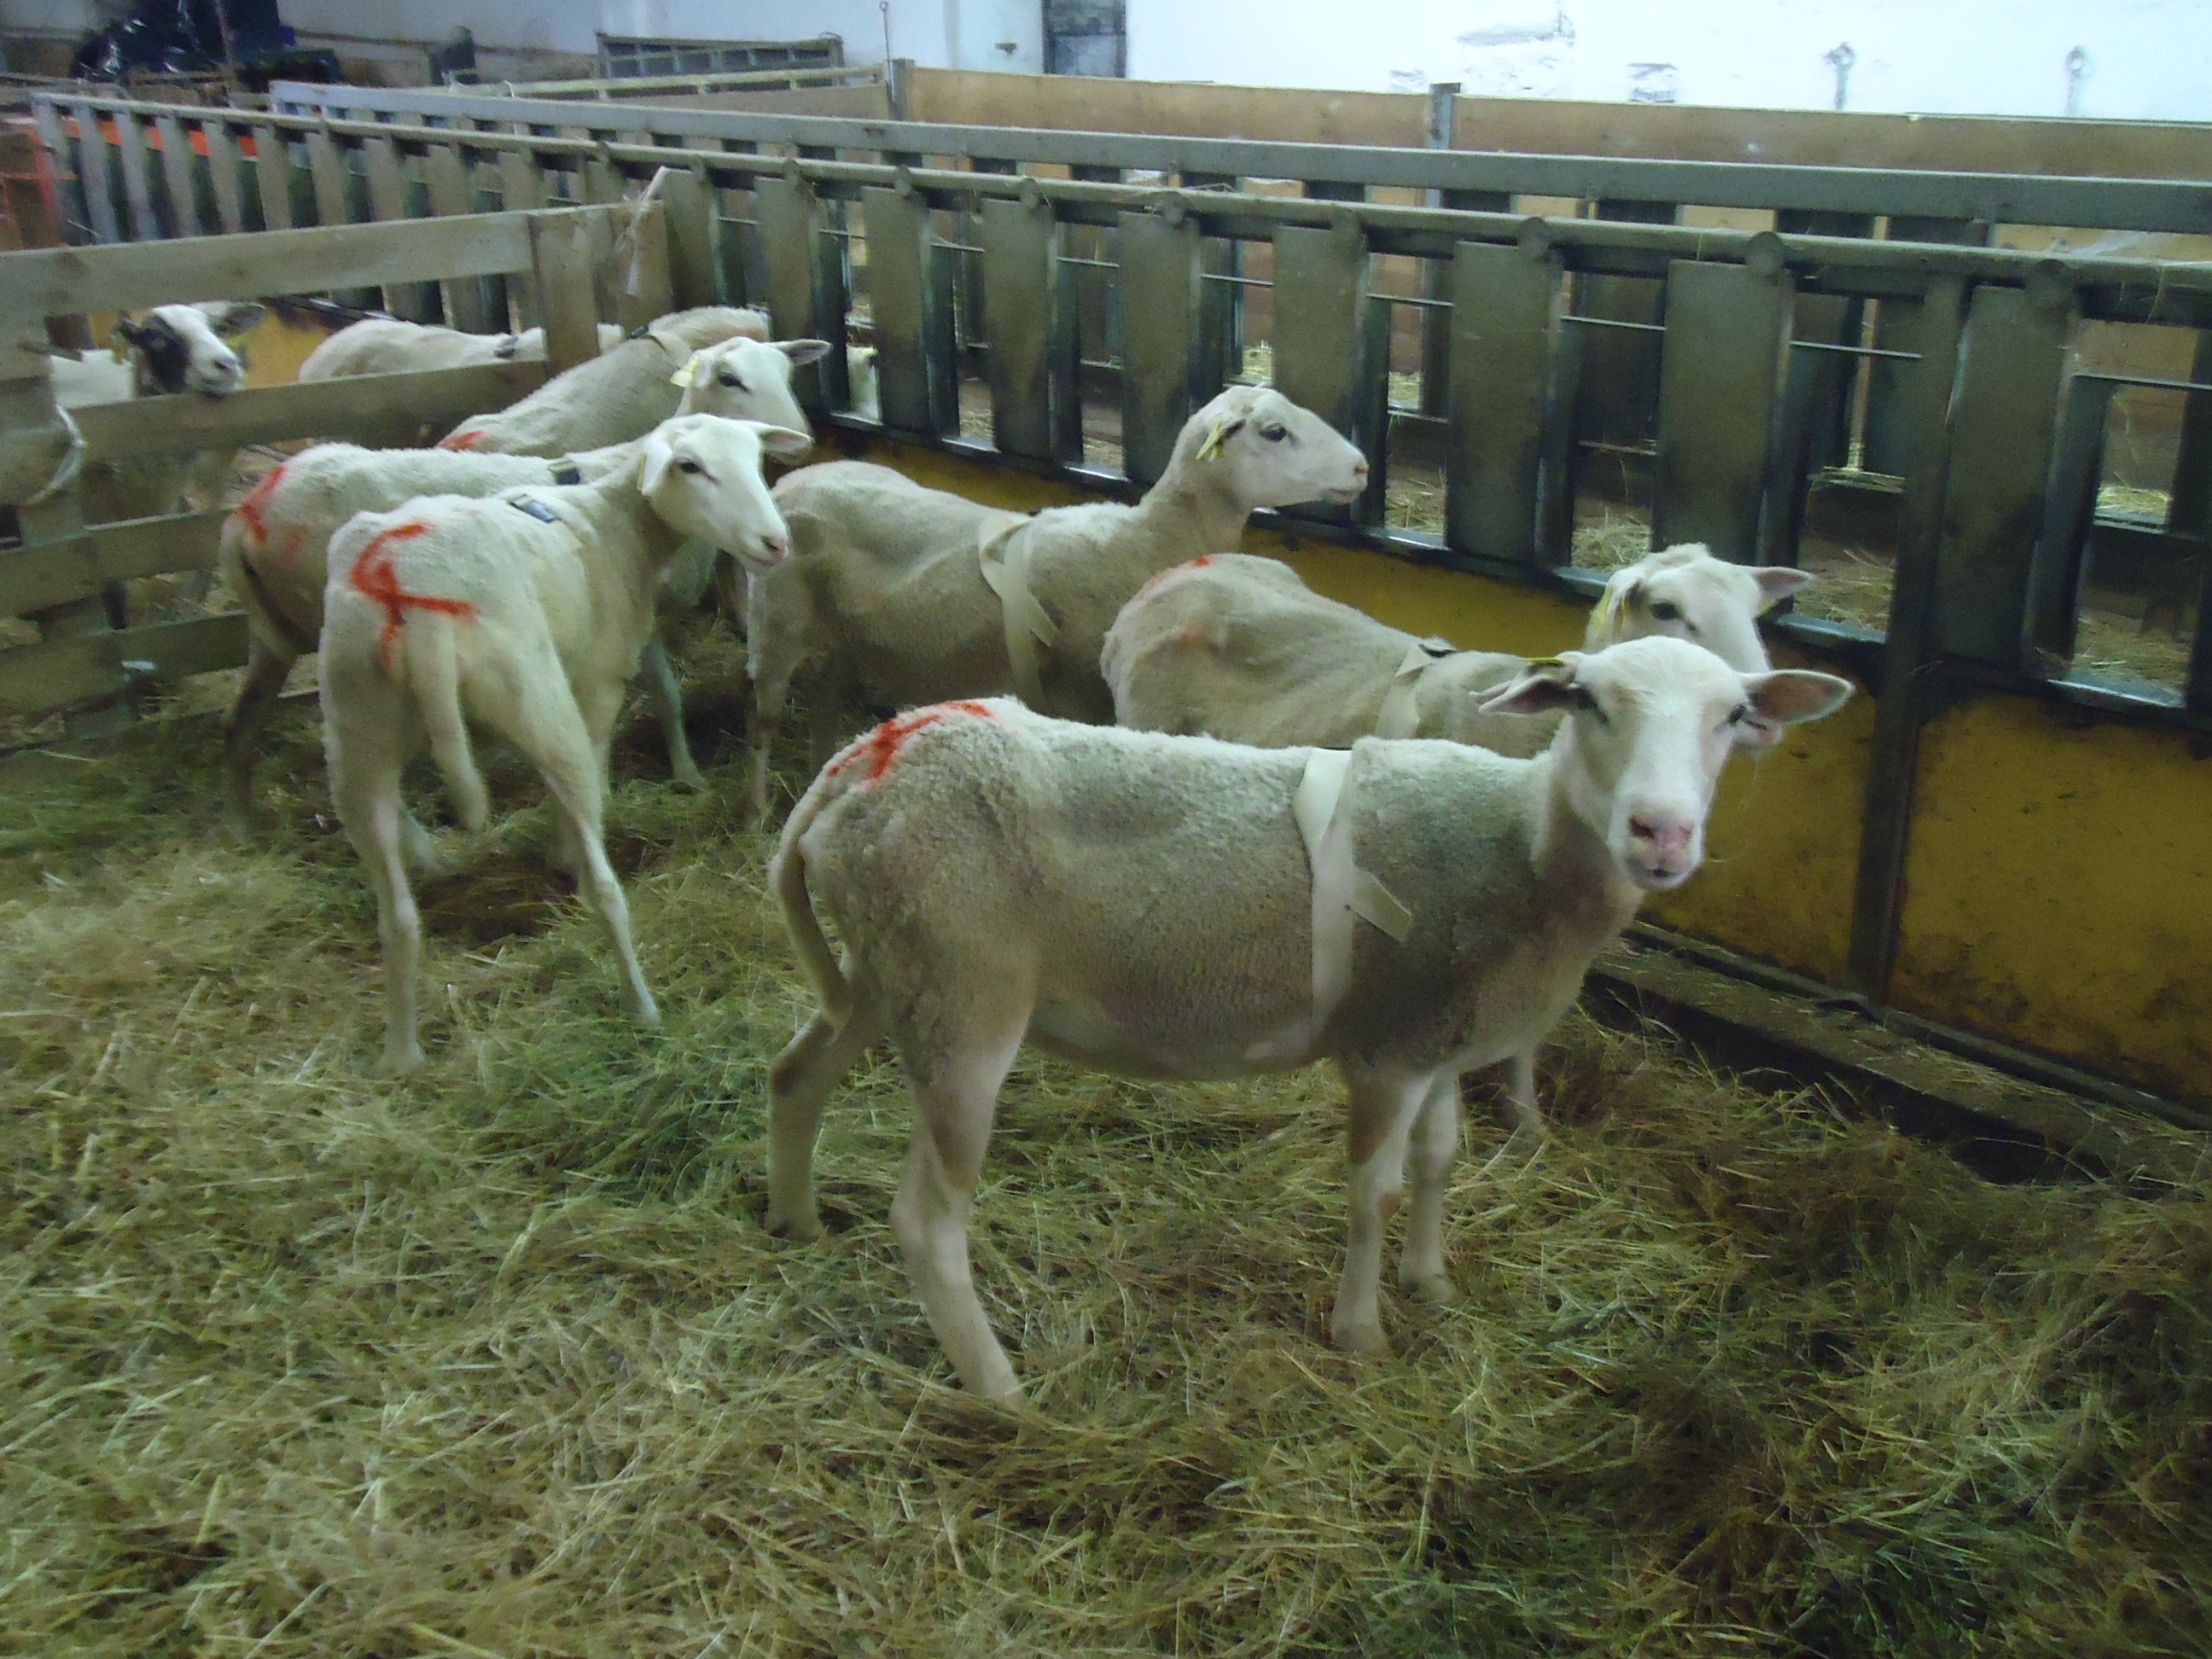
\includegraphics[width=0.7\linewidth]{./img/animais} 

}

\caption{Fotografia dos animais sob análise.}\label{fig:unnamed-chunk-3}
\end{figure}

\endColumns
\end{frame}

\begin{frame}{Estudo de caso}
\protect\hypertarget{estudo-de-caso-2}{}
\begin{figure}

{\centering 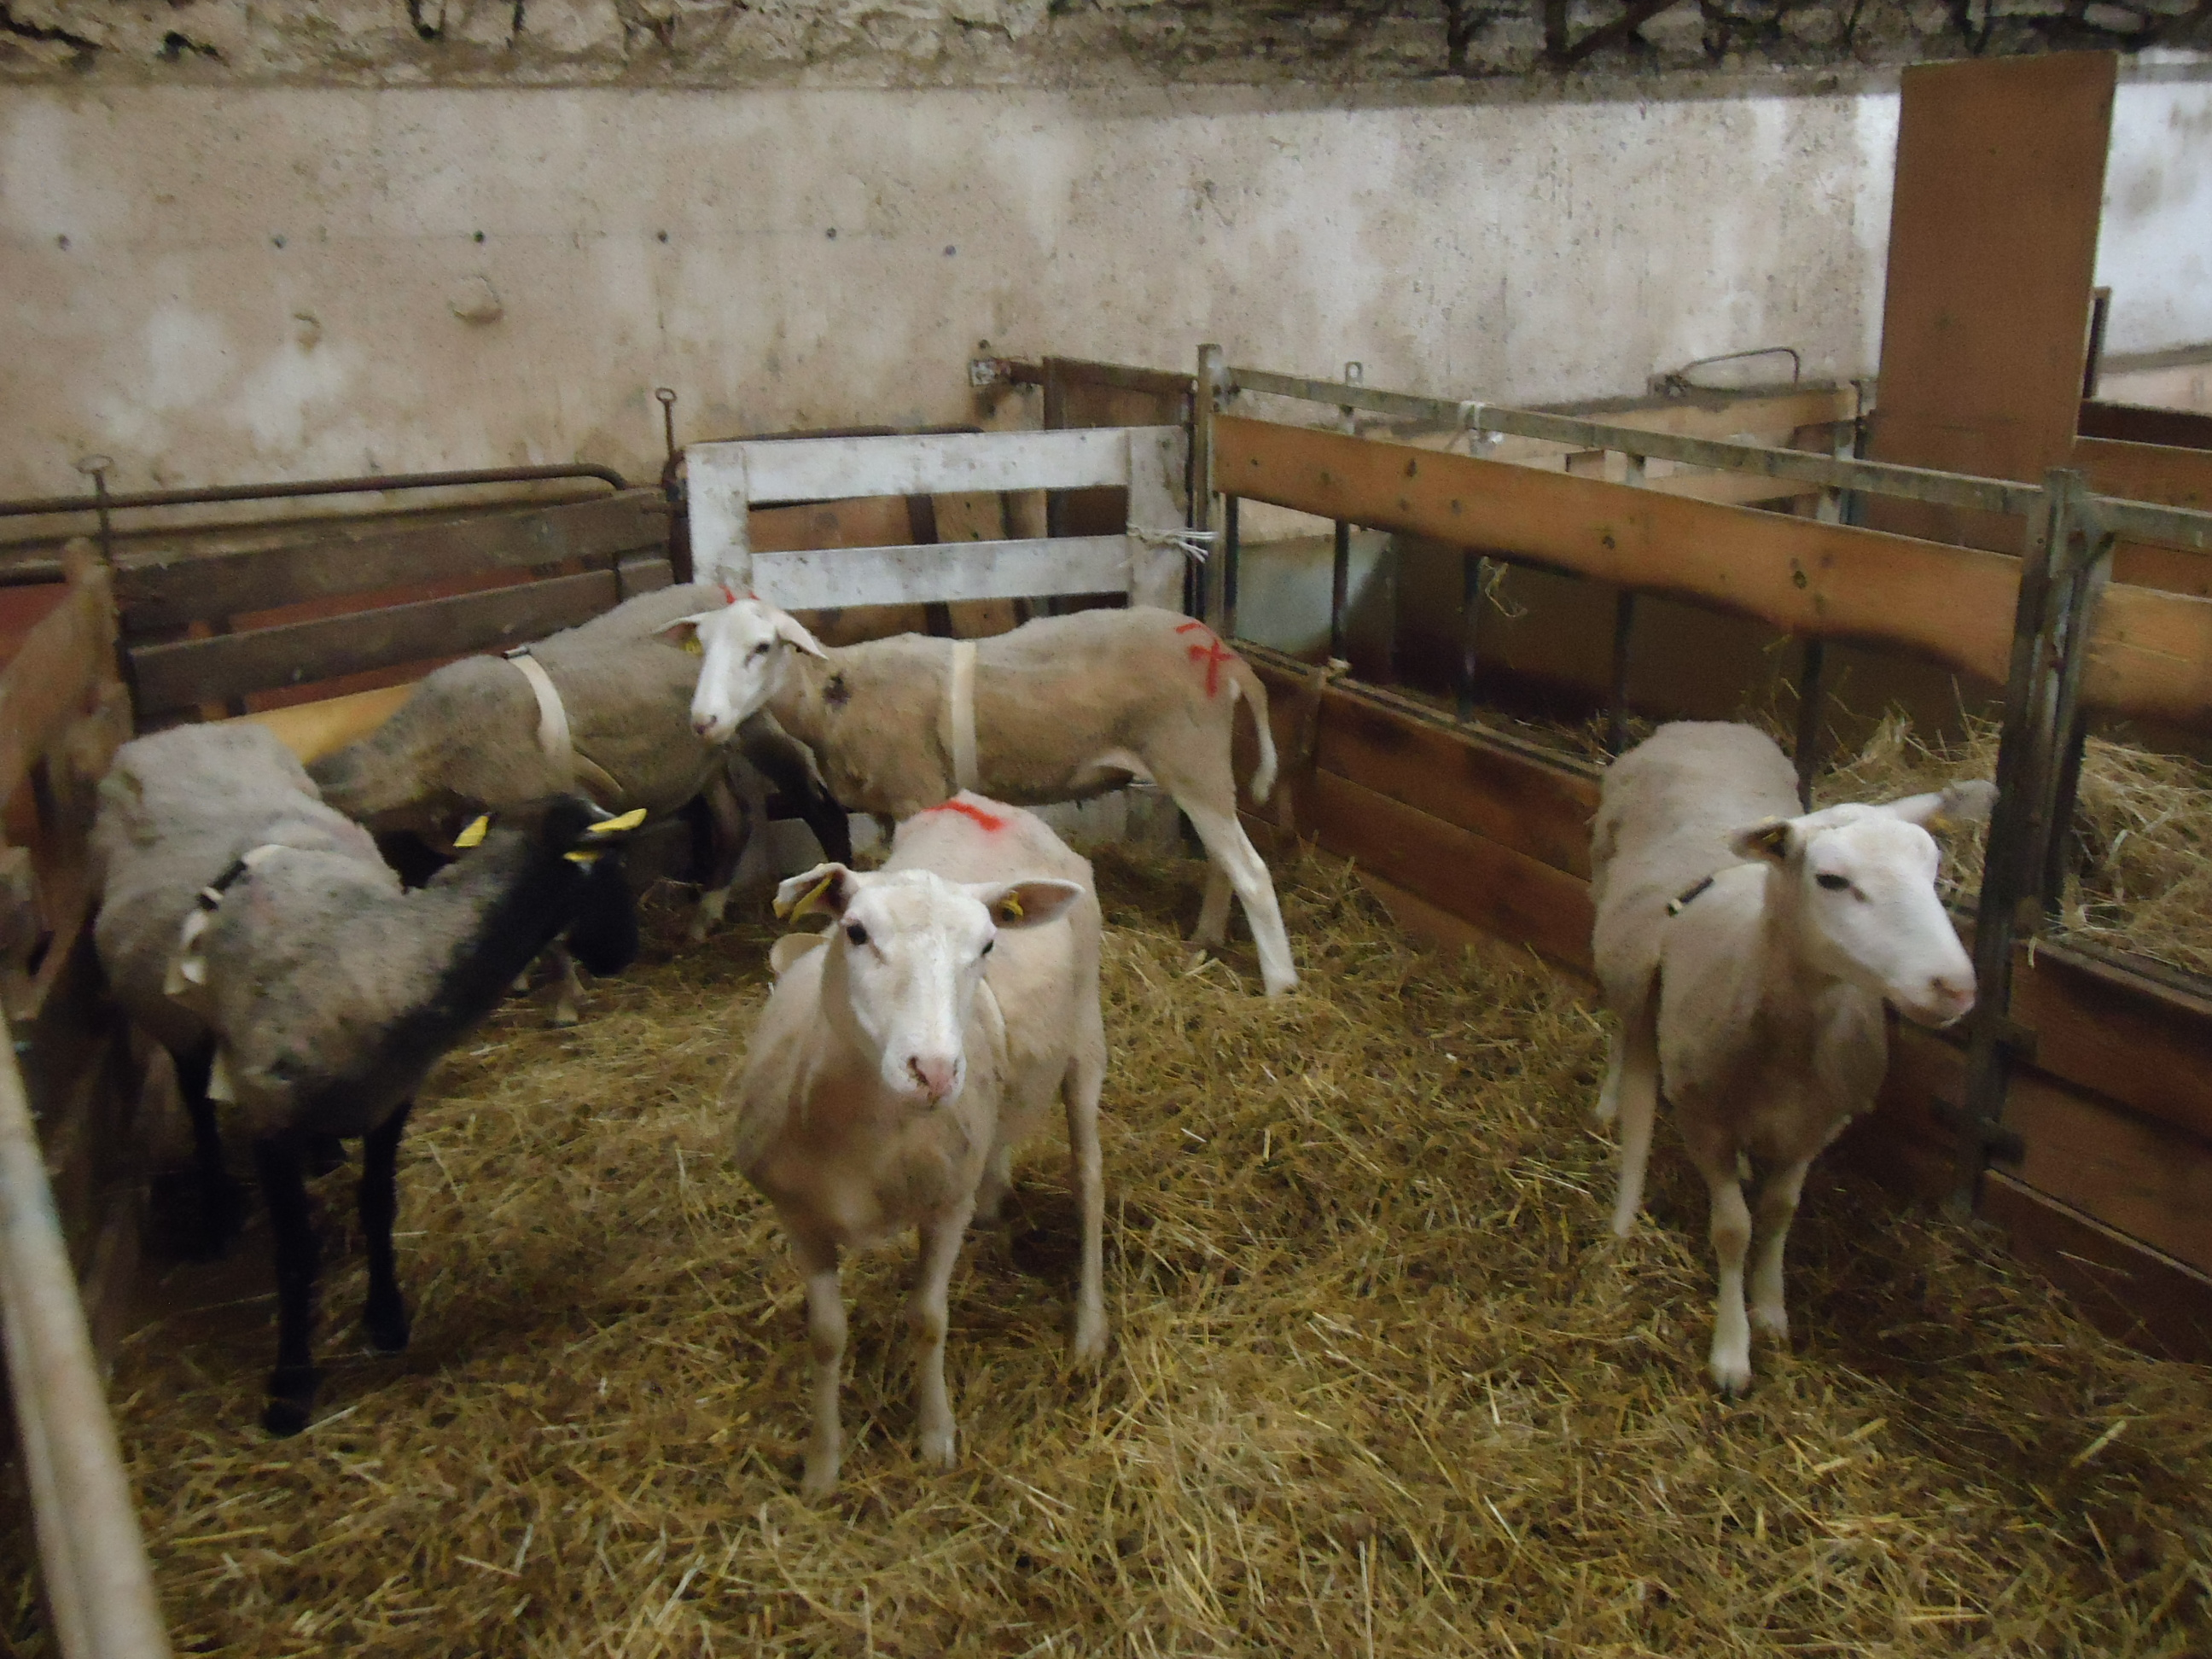
\includegraphics[width=0.55\linewidth]{./img/animais2} 

}

\caption{Fotografia dos animais sob análise.}\label{fig:unnamed-chunk-4}
\end{figure}
\end{frame}

\begin{frame}{Estudo de caso}
\protect\hypertarget{estudo-de-caso-3}{}
O experimento foi conduzido em \textbf{três sessões experimentais}:

\begin{enumerate}
\item
  Na primeira havia uma grade de metal separando o animal testado dos
  demais animais, \textbf{sem distância} entre eles.
\item
  Na segunda havia duas grades de metal separando o animal testado dos
  demais animais a uma \textbf{distância de 1,7 m}.
\item
  Na terceira sessão os animais voltaram a ser separados por apenas uma
  grade, \textbf{sem distanciamento} dos demais animais.
\end{enumerate}
\end{frame}

\begin{frame}{Estudo de caso}
\protect\hypertarget{estudo-de-caso-4}{}
\begin{figure}

{\centering \includegraphics[width=0.7\linewidth]{./img/se1_se3} 

}

\caption{Esquema sessões 1 e 3 (sem isolamento).}\label{fig:unnamed-chunk-5}
\end{figure}
\end{frame}

\begin{frame}{Estudo de caso}
\protect\hypertarget{estudo-de-caso-5}{}
\begin{figure}

{\centering \includegraphics[width=0.7\linewidth]{./img/se2} 

}

\caption{Esquema sessão 2 (com isolamento).}\label{fig:unnamed-chunk-6}
\end{figure}
\end{frame}

\begin{frame}{Estudo de caso}
\protect\hypertarget{estudo-de-caso-6}{}
\begin{figure}

{\centering 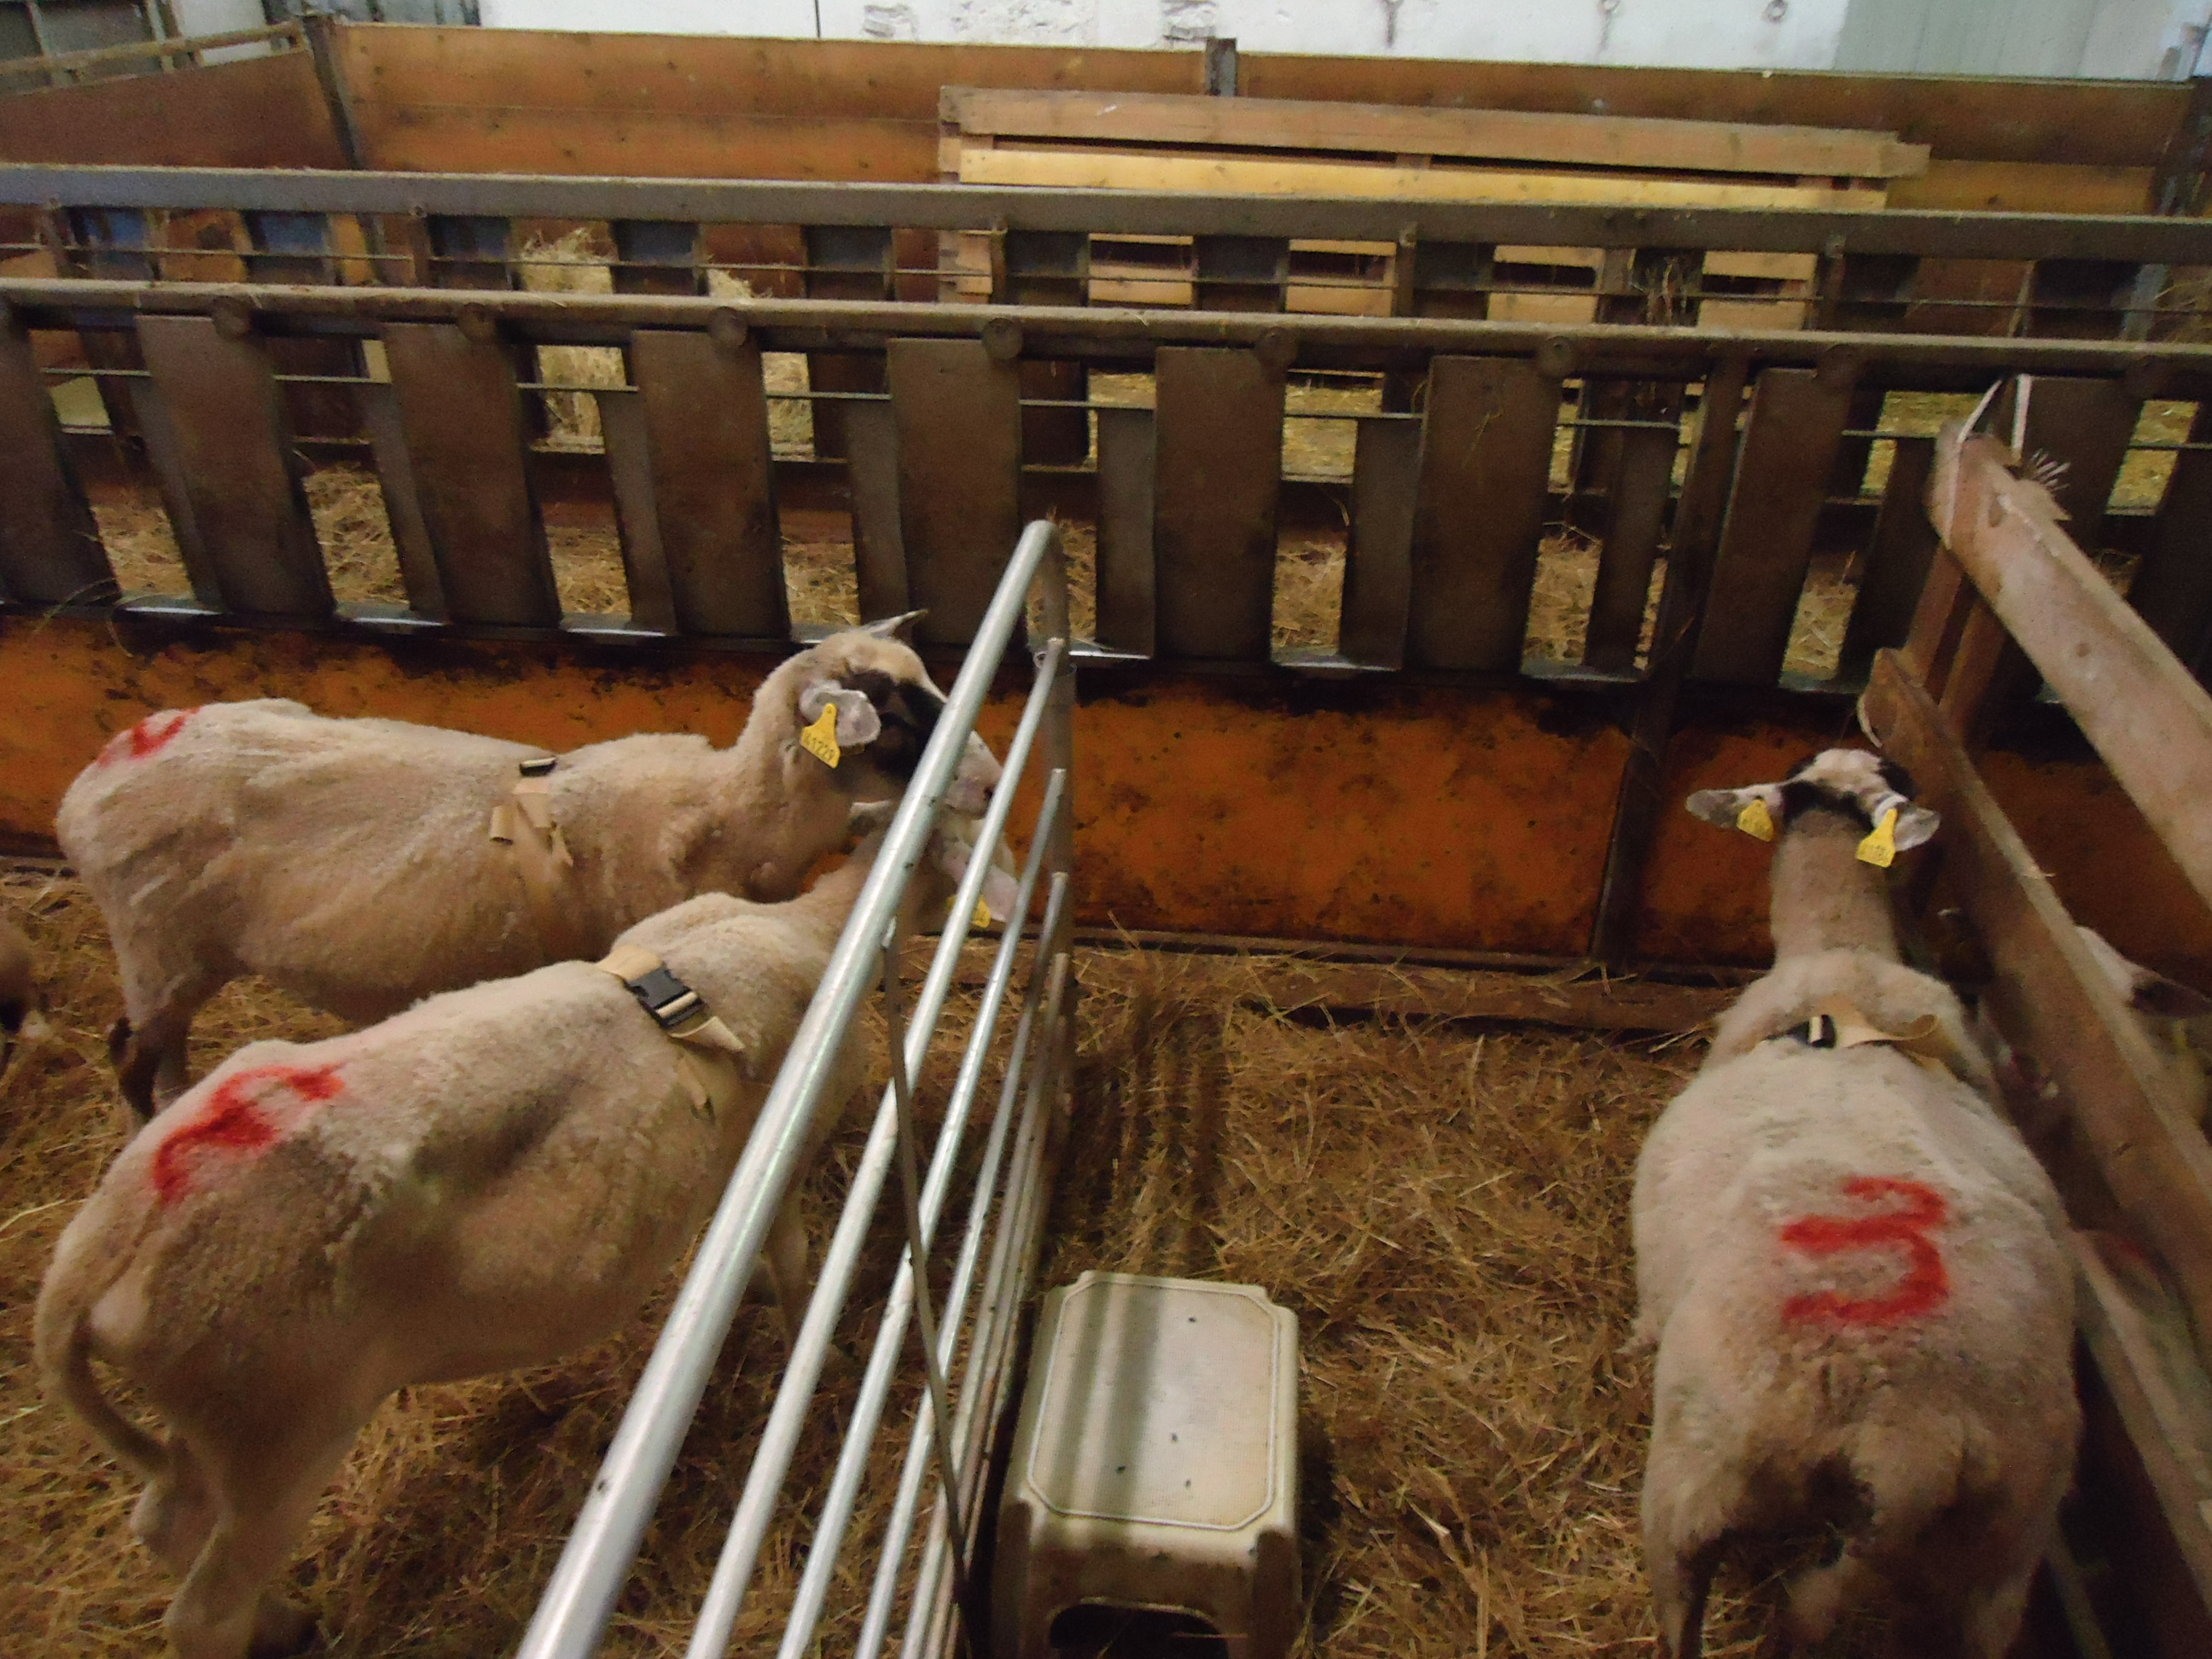
\includegraphics[width=0.55\linewidth]{./img/isol} 

}

\caption{Fotografia sessão sem isolamento.}\label{fig:unnamed-chunk-7}
\end{figure}
\end{frame}

\begin{frame}{Estudo de caso}
\protect\hypertarget{estudo-de-caso-7}{}
Em cada sessão, as ovelhas foram observadas em \textbf{3 momentos}
distintos:

\begin{enumerate}
\item
  Fase de \textbf{pré escovação}, com duração de 2 minutos e 30
  segundos.
\item
  Fase de \textbf{escovação}, com duração de 3 minutos.
\item
  Fase de \textbf{pós escovação}, com duração de 2 minutos e 30
  segundos.
\end{enumerate}
\end{frame}

\begin{frame}{Estudo de caso}
\protect\hypertarget{estudo-de-caso-8}{}
\begin{figure}

{\centering 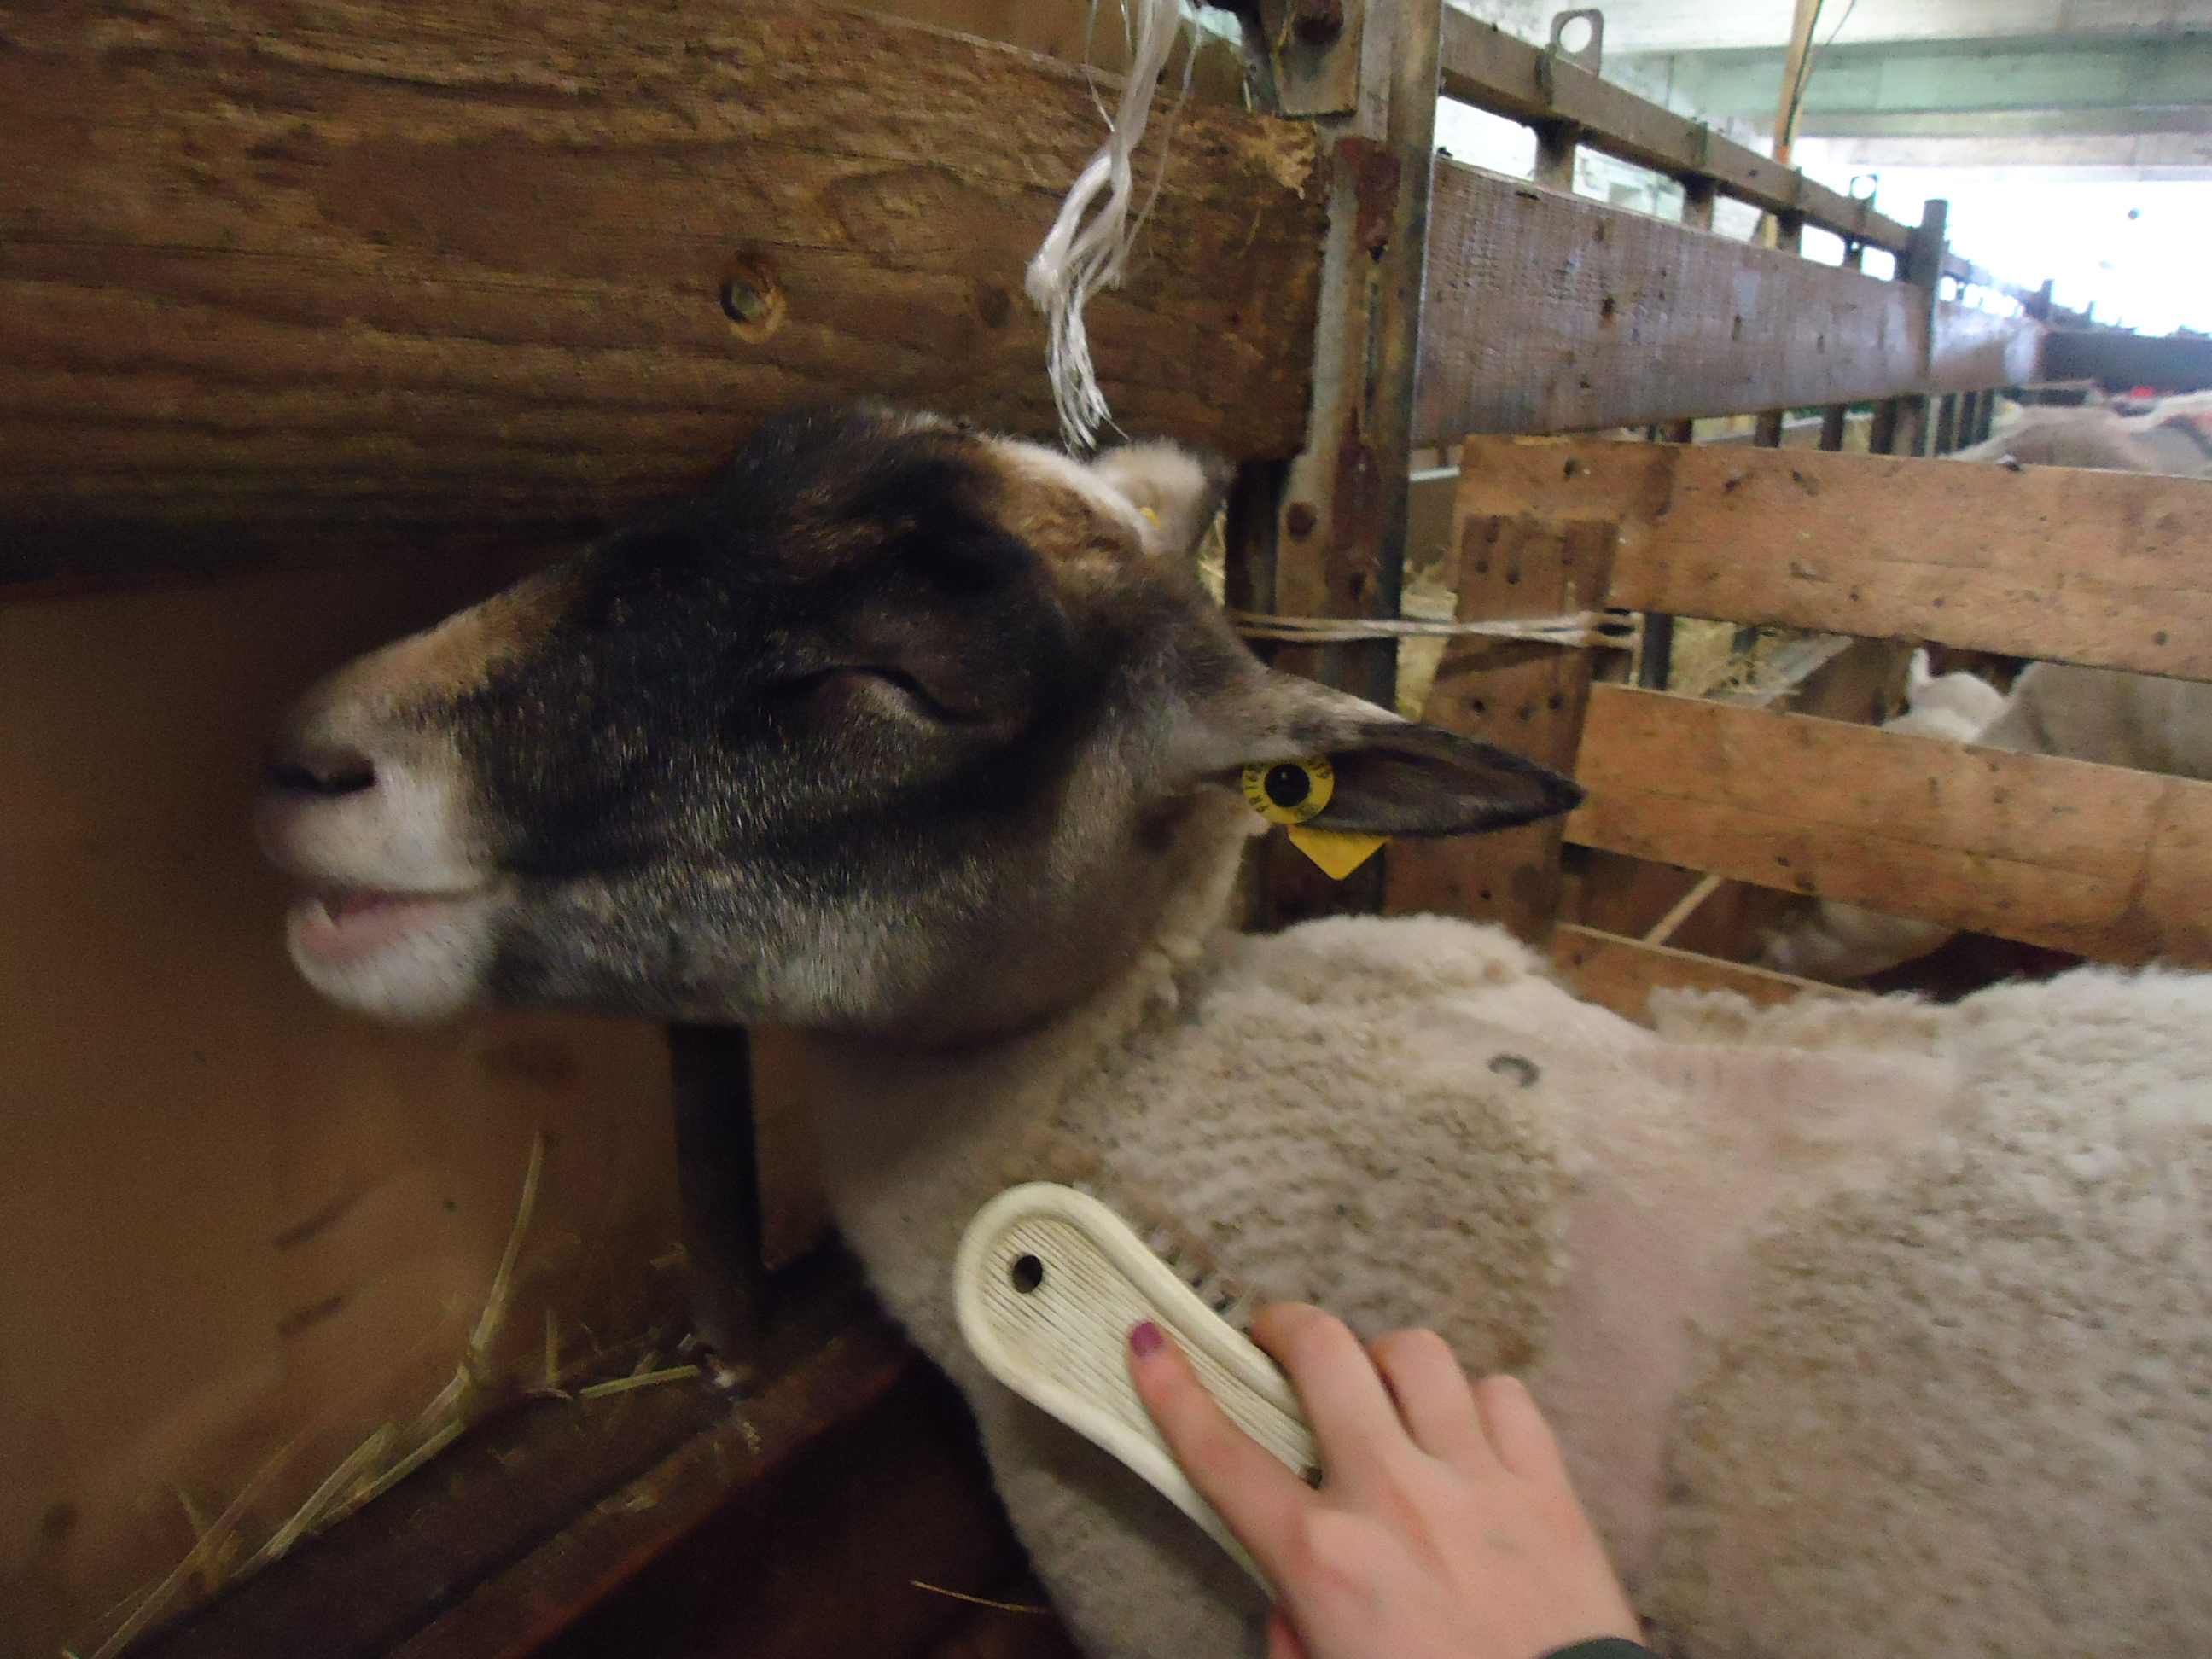
\includegraphics[width=0.55\linewidth]{./img/escov} 

}

\caption{Fotografia animal sob intervenção humana (escovação).}\label{fig:unnamed-chunk-8}
\end{figure}
\end{frame}

\begin{frame}{Estudo de caso}
\protect\hypertarget{estudo-de-caso-9}{}
Temos \textbf{3 variáveis categóricas}:

\begin{enumerate}
\item
  \textbf{Linhagem}: fator de 2 níveis que classifica os animais como
  reativos (R+) ou não reativos (R-).
\item
  \textbf{Sessão}: fator de 3 níveis que indica a sessão experimental de
  acordo com o isolamento social (sessões 1 e 3 sem isolamento, sessão 2
  com isolamento).
\item
  \textbf{Momento}: fator de 3 níveis que indica se o animal está ou não
  sob intervenção humana (antes, durante ou depois da intervenção).
\end{enumerate}

Temos \textbf{2 respostas} distintas:

\begin{enumerate}
\tightlist
\item
  Número de mudanças de postura de orelha.
\item
  Proporção do tempo com as orelhas em posição neutra.
\end{enumerate}
\end{frame}

\begin{frame}{Estudo de caso}
\protect\hypertarget{estudo-de-caso-10}{}
\begin{itemize}
\item
  Considerando as combinações entre as variáveis, \textbf{cada animal}
  contribui com \textbf{9 medidas} ao conjunto de dados.
\item
  Portanto existe uma estrutura de medidas repetidas.
\end{itemize}

\begin{figure}

{\centering \includegraphics[width=0.55\linewidth]{./img/se_mo} 

}

\caption{Combinação entre sessão e momento.}\label{fig:unnamed-chunk-9}
\end{figure}
\end{frame}

\hypertarget{gamlss-2}{%
\section{GAMLSS}\label{gamlss-2}}

\begin{frame}{GAMLSS}
\protect\hypertarget{gamlss-3}{}
Para definição de um GAMLSS considere:

\begin{itemize}
\item
  Um conjunto de observações \(Y_i, \ i=1,2,\ldots,n\).
\item
  As observações seguem função (densidade) de probabilidade
  \(f_Y(y_i|\theta)\) parametrizada por
  \(\theta = (\theta_{1}, ..., \theta_{p})^T\).
\item
  \(\theta\) é um vetor de \(p\) até 4 parâmetros distribucionais
  denotados por \((\mu, \sigma, \nu, \tau)^T\) se \(p=4\).
\item
  Geralmente (mas não necessariamente) \(\mu\) e \(\sigma\) representam
  os parâmetros de locação e dispersão, enquanto que \(\nu\) and
  \(\tau\) representam parâmetros de forma.
\end{itemize}
\end{frame}

\begin{frame}{GAMLSS}
\protect\hypertarget{gamlss-4}{}
\begin{equation}\label{eq.gamlss}
    \begin{aligned}
        g_{k}(\theta_{k}) = \eta_{k} = X_{k} \beta_{k} + \sum_{j=1}^{J_{k}} Z_{jk} \gamma_{jk},\ k=1,2,3,4,
    \end{aligned}
\end{equation}

\begin{itemize}
\item
  \(g_{k}(\cdot)\) são funções de ligação que relacionam o \(k\)-ésimo
  parâmetro distribucional ao preditor \(\eta_{k}\).
\item
  \(\beta_{k} = (\beta_{1k},\beta_{2k},\ldots,\beta_{J_{K}^{'}k})^T\) é
  um vetor de parâmetros de regressão de dimensão \(J_{K}^{'}\),
\item
  \(X_{k}\) e \(Z_{jk}\) são matrizes de delineamento de ordem
  \(n \times J_{k}^{'}\) e \(n \times q_{jk}\), respectivamente.
\item
  \(\gamma_{jk}\) é um vetor aleatório de dimensão \(q_{jk}\) para os
  quais assume-se que
  \(\gamma_{jk} \sim \text{N}_{q_{jk}}(0, G_{jk}^{-1})\).
\item
  \(G_{jk}^{-1}\) é a inversa generalizada da matriz simétrica
  \(G_{jk} = G_{jk}(\lambda_{jk})\) de ordem \(q_{jk} \times q_{jk}\)
\item
  \(\lambda_{jk}\) é um vetor de hiperparâmetros.
\end{itemize}
\end{frame}

\begin{frame}{GAMLSS}
\protect\hypertarget{gamlss-5}{}
\begin{itemize}
\tightlist
\item
  Os parâmetros de regressão (\(\beta_{k}\)) e os efeitos aleatórios
  (\(\gamma_{jk}\)) são usualmente estimados na maximização de uma
  log-verossimilhança penalizada (\(l_p\)), dada por
\end{itemize}

\begin{equation}\label{eq.loglik}
    \begin{aligned}
        l_p = l-\frac{1}{2} \sum_{k=1}^{p} \sum_{j=1}^{J_k} \lambda_{jk} \gamma_{jk}^{'} G_{jk} \gamma_{jk},
    \end{aligned}
\end{equation}

\begin{itemize}
\item
  \(l = \sum_{i=1}^{n} \log(f(y_i|\theta))\) representa a
  log-verossimilhança.
\item
  A log-verossimilhança penalizada se reduz à usual log-verossimilhança
  quando não há efeitos aleatórios ou termos suavizadores no modelo.
\end{itemize}
\end{frame}

\hypertarget{aplicauxe7uxe3o}{%
\section{Aplicação}\label{aplicauxe7uxe3o}}

\begin{frame}{Procedimento de análise}
\protect\hypertarget{procedimento-de-anuxe1lise}{}
\textbf{Respostas}

\begin{enumerate}
\tightlist
\item
  Número de mudanças de postura de orelha.
\item
  Proporção do tempo com as orelhas em posição neutra.
\end{enumerate}

\textbf{Procedimento}

\begin{enumerate}
\tightlist
\item
  Seleção de distribuições compatíveis com o problema.
\item
  Ajuste de modelos com o mesmo preditor para todas as distribuições.
\item
  Seleção do modelos via medidas de qualidade de ajuste OU análise
  gráfica.
\item
  Busca do menor modelo possível que não fosse estatisticamente
  diferente do modelo inicial.
\item
  Interpretação dos resultados.
\end{enumerate}
\end{frame}

\hypertarget{nuxfamero-de-mudanuxe7as-de-postura-de-orelha}{%
\section{Número de mudanças de postura de
orelha}\label{nuxfamero-de-mudanuxe7as-de-postura-de-orelha}}

\begin{frame}{Análise exploratória}
\protect\hypertarget{anuxe1lise-exploratuxf3ria}{}
\begin{figure}

{\centering 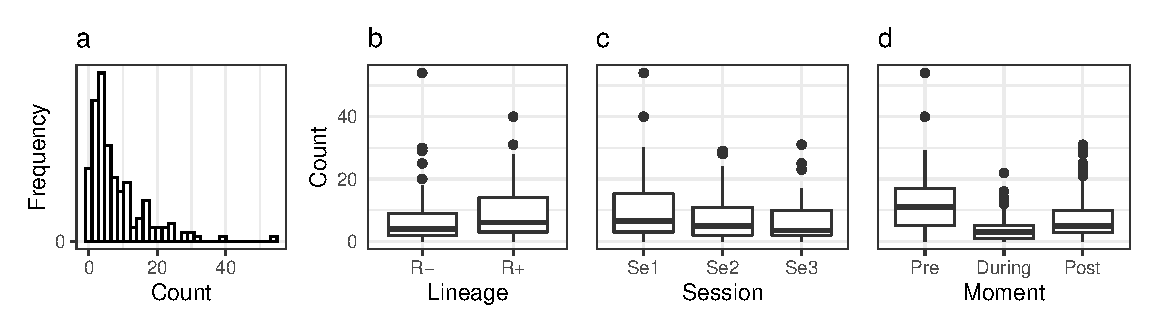
\includegraphics[width=0.95\linewidth]{./img/count} 

}

\caption{Análise exploratória do número de mudanças de postura de orelha.}\label{fig:unnamed-chunk-10}
\end{figure}
\end{frame}

\begin{frame}{Distribuições}
\protect\hypertarget{distribuiuxe7uxf5es}{}
\begin{itemize}
\tightlist
\item
  Poisson (\textbf{PO}).
\item
  Negative binomial distribution (\textbf{NBI}).
\item
  Zero inflated Poisson distribution (\textbf{ZIP}).
\item
  Zero inflated negative binomial distribution (\textbf{ZINBI}).
\item
  Zero adjusted Poisson distribution (\textbf{ZAP}).
\item
  Zero adjusted negative binomial distribution (\textbf{ZANBI}).
\end{itemize}
\end{frame}

\begin{frame}{Preditores iniciais}
\protect\hypertarget{preditores-iniciais}{}
\begin{itemize}
\item
  Para cada distribuição os modelos foram especificados com os efeitos
  fixos de \textbf{sessão}, \textbf{momento}, \textbf{linhagem} e as
  \textbf{interações duas a duas}.
\item
  Adicionalmente foram incluídos 2 \textbf{efeitos aleatórios}: um a
  nível de \textbf{animal} e outro a nível de
  \textbf{animal dentro de sessão}.
\item
  Nas distribuições com parâmetros associados à
  \textbf{inflação de zeros} foram incluídos os efeitos fixos de
  \textbf{sessão}, \textbf{momento} e \textbf{linhagem}.
\end{itemize}
\end{frame}

\begin{frame}{Seleção de modelos}
\protect\hypertarget{seleuxe7uxe3o-de-modelos}{}
\begin{itemize}
\item
  A distribuição foi selecionada por meio de
  \textbf{medidas de qualidade de ajuste}.
\item
  A distribuição com melhor desempenho foi a \textbf{ZANBI}.
\item
  Buscou-se o \textbf{menor modelo} que não diferisse do original.

  \begin{itemize}
  \tightlist
  \item
    Testou-se a \textbf{exclusão de variáveis} explicativas do modelo.
  \item
    A comparação entre o modelo original e os reduzidos foi feito por
    meio do \textbf{teste da razão de verossimilhanças}.
  \end{itemize}
\end{itemize}
\end{frame}

\begin{frame}{Especificação}
\protect\hypertarget{especificauxe7uxe3o}{}
Considere \(Y_{ijkl}\) a variável resposta.

\begin{itemize}
\item
  \(i\ (i=1,2,\ldots,20)\) representa o animal.
\item
  \(j\ (j=1,2,3)\) representa a sessão.
\item
  \(k\ (k=1,2,3)\) representa o momento.
\item
  \(l\) \((l=1,2)\) representa a linhagem.
\end{itemize}
\end{frame}

\begin{frame}{Especificação}
\protect\hypertarget{especificauxe7uxe3o-1}{}
\begin{equation}
    \begin{aligned}
        Y_{ijkl}|u_{j},v_{jk} \sim\,  ZANBI(\mu_{ijkl}, \sigma, \nu_{ikl}),
    \end{aligned}
    \label{eq.model.geral}
\end{equation}

\begin{itemize}
\item
  \(\mu_{ijkl}\) representa o parâmetro de locação da distribuição
  condicional de \(y\).
\item
  \(\sigma\) representa o parâmetro de dispersão.
\item
  \(\nu_{ikl}\) está associado ao excesso de zeros.
\item
  \(u_{i}\) representa o efeito aleatório a nível de animal.

  \begin{itemize}
  \tightlist
  \item
    \(u_{i} \sim \text{N}(0, \sigma^{2}_{U})\)
  \end{itemize}
\item
  \(v_{ik}\) representa o efeito aleatório a nível de animal dentro de
  sessão.

  \begin{itemize}
  \tightlist
  \item
    \(v_{ik} \sim \text{N}(0, \sigma^{2}_{V})\)
  \end{itemize}
\end{itemize}
\end{frame}

\begin{frame}{Modelo final}
\protect\hypertarget{modelo-final}{}
\begin{equation}
    \begin{aligned}
        \log(\mu_{ijkl}) = \alpha^{(1)} + \beta_{j}^{(1)} + \gamma_{k}^{(1)} + \theta_{l}^{(1)} + u_{i} + v_{ik}
    \end{aligned}
    \label{eq.count.mu}
\end{equation}

\begin{equation}
    \begin{aligned}
        \text{logit}(\nu_{jkl}) = \alpha^{(2)} + \beta_{j}^{(2)} + \gamma_{k}^{(2)} + \theta_{l}^{(2)}
    \end{aligned}
    \label{eq.count.nu}
\end{equation}

\begin{itemize}
\tightlist
\item
  \(\alpha^{(1)}\) representa o intercepto.
\item
  \(\beta_{j}^{(1)}\) representa o efeito de sessão.
\item
  \(\gamma_{k}^{(1)}\) representa o efeito de momento.
\item
  \(\theta_{l}^{(1)}\) representa o efeito de linhagem.
\end{itemize}
\end{frame}

\begin{frame}{Diagnóstico}
\protect\hypertarget{diagnuxf3stico}{}
\begin{figure}

{\centering \includegraphics[width=0.95\linewidth]{./img/mzanbi} 

}

\caption{Análise dos resíduos quantílicos aleatorizados do modelo ZANBI final.}\label{fig:unnamed-chunk-11}
\end{figure}
\end{frame}

\begin{frame}{Estimativas}
\protect\hypertarget{estimativas}{}
\begin{table}[h]
    \centering
    \caption{Relative rates, odds ratios, confidence intervals and p-values for the final \text{ZANBI} model. Session 1, moment before brushing and lineage $R-$ are taken as reference categories}
    \begin{tabular}{lcclccc}
        \hline
        & \multicolumn{3}{c}{$\mu$}                                                                                                         & \multicolumn{3}{c}{$\nu$}                                                                                                        \\ \hline
        \multicolumn{1}{l|}{Parm.}           & RR                    & CI(95\%)                             & \multicolumn{1}{c|}{P-value}                                & OR                    & CI(95\%)                             & P-value                                                    \\ \hline
        \multicolumn{1}{l|}{$\alpha$}        & {\color[HTML]{000000} 15.77} & {\color[HTML]{000000} (13.12; 18.95)} & \multicolumn{1}{c|}{{\color[HTML]{000000} \textless{}0.001}} & {\color[HTML]{000000} 0.004} & {\color[HTML]{000000} (0.00; 0.06)}   & \multicolumn{1}{l}{{\color[HTML]{000000} \textless{}0.001}} \\
        \multicolumn{1}{l|}{$\beta_{se2}$}   & {\color[HTML]{000000} 0.69}  & {\color[HTML]{000000} (0.56; 0.84)}   & \multicolumn{1}{l|}{{\color[HTML]{000000} \textless{}0.001}} & {\color[HTML]{000000} 5.83}  & {\color[HTML]{000000} (0.64; 53.54)}  & {\color[HTML]{000000} 0.121}                                \\
        \multicolumn{1}{l|}{$\beta_{se3}$}   & {\color[HTML]{000000} 0.66}  & {\color[HTML]{000000} (0.53; 0.81)}   & \multicolumn{1}{l|}{{\color[HTML]{000000} \textless{}0.001}} & {\color[HTML]{000000} 14.31} & {\color[HTML]{000000} (1.69; 121.49)} & \multicolumn{1}{l}{{\color[HTML]{000000}\   0.016}} \\
        \multicolumn{1}{l|}{$\gamma_{dur}$}  & {\color[HTML]{000000} 0.35}  & {\color[HTML]{000000} (0.28; 0.43)}   & \multicolumn{1}{l|}{{\color[HTML]{000000} \textless{}0.001}} & {\color[HTML]{000000} 15.80} & {\color[HTML]{000000} (1.89; 131.99)} & \multicolumn{1}{l}{{\color[HTML]{000000} \ 0.012}} \\
        \multicolumn{1}{l|}{$\gamma_{post}$} & {\color[HTML]{000000} 0.65}  & {\color[HTML]{000000} (0.54; 0.79)}   & \multicolumn{1}{l|}{{\color[HTML]{000000} \textless{}0.001}} & {\color[HTML]{000000} 4.43}  & {\color[HTML]{000000} (0.47; 42.12)}  & {\color[HTML]{000000} 0.197}                                \\
        \multicolumn{1}{l|}{$\theta_{R+}$}   & {\color[HTML]{000000} 1.33}  & {\color[HTML]{000000} (1.12; 1.57)}   & \multicolumn{1}{l|}{{\color[HTML]{000000} \ \  0.001}} & {\color[HTML]{000000} 0.33}  & {\color[HTML]{000000} (0.09; 1.14)}   & {\color[HTML]{000000} 0.081}                                \\ \hline
    \end{tabular}
    \label{tab:est1}
\end{table}
\end{frame}

\begin{frame}{Interpretação}
\protect\hypertarget{interpretauxe7uxe3o}{}
\textbf{Os animais apresentaram }

\begin{itemize}
\item
  Menores contagens nas sessões 2 e 3 quando comparados com a sessão 1.
\item
  Menores contagens durante e depois da intervenção quando comparados
  com antes.
\item
  Maiores contagens são observadas em animais reativos.
\end{itemize}

\textbf{Sobre a propensão a não mover as orelhas}

\begin{itemize}
\item
  Durante a escovação os animais são mais propensos a não mover as
  orelhas.
\item
  Animais não reativos são mais propensos a não mover as orelhas.
\end{itemize}
\end{frame}

\hypertarget{proporuxe7uxe3o-do-tempo-com-as-orelhas-em-posiuxe7uxe3o-neutra}{%
\section{Proporção do tempo com as orelhas em posição
neutra}\label{proporuxe7uxe3o-do-tempo-com-as-orelhas-em-posiuxe7uxe3o-neutra}}

\begin{frame}{Análise exploratória}
\protect\hypertarget{anuxe1lise-exploratuxf3ria-1}{}
\begin{figure}

{\centering 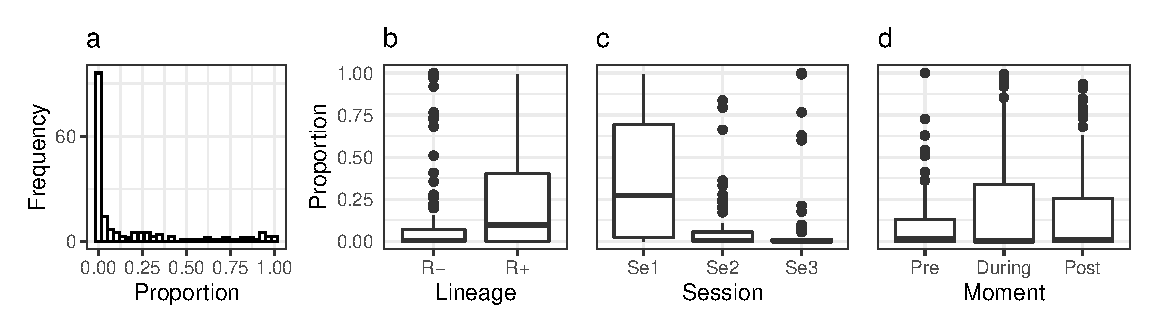
\includegraphics[width=0.95\linewidth]{./img/prop} 

}

\caption{Análise exploratória da proporção do tempo com as orelhas em posição neutra.}\label{fig:unnamed-chunk-12}
\end{figure}
\end{frame}

\begin{frame}{}
\protect\hypertarget{section}{}
\textbf{Distribuições}

\begin{itemize}
\tightlist
\item
  Beta (\textbf{BE}).
\item
  Beta inflacionada (\textbf{BEINF}).
\end{itemize}

\vspace{0.5cm}

\textbf{Preditores iniciais}

\begin{itemize}
\item
  Para cada distribuição os modelos foram especificados com os efeitos
  fixos de \textbf{sessão}, \textbf{momento}, \textbf{linhagem} e as
  \textbf{interações duas a duas}.
\item
  Adicionalmente foram incluídos 2 \textbf{efeitos aleatórios}: um a
  nível de \textbf{animal} e outro a nível de
  \textbf{animal dentro de sessão}.
\item
  Na distribuição Beta Inflacionada, foram incluídos os efeitos fixos de
  \textbf{sessão}, \textbf{momento} e \textbf{linhagem} no parâmetro
  referente à inflação de zeros.
\end{itemize}
\end{frame}

\begin{frame}{Seleção de modelos}
\protect\hypertarget{seleuxe7uxe3o-de-modelos-1}{}
\begin{itemize}
\item
  A distribuição foi selecionada por meio da
  \textbf{análise gráfica dos resíduos quantílicos aleatorizados}.
\item
  A distribuição com melhor desempenho foi a \textbf{BEINF}.
\item
  Buscou-se o \textbf{menor modelo} que não diferisse do original.

  \begin{itemize}
  \tightlist
  \item
    Testou-se a \textbf{exclusão de variáveis} explicativas do modelo.
  \item
    A comparação entre o modelo original e os reduzidos foi feito por
    meio do \textbf{teste da razão de verossimilhanças}.
  \end{itemize}
\end{itemize}
\end{frame}

\begin{frame}{Seleção de modelos}
\protect\hypertarget{seleuxe7uxe3o-de-modelos-2}{}
\begin{figure}

{\centering \includegraphics[width=0.9\linewidth]{./img/mbetas} 

}

\caption{Análise dos resíduos quantílicos aleatorizados para os modelos Beta e Beta Inflacionado.}\label{fig:unnamed-chunk-13}
\end{figure}
\end{frame}

\begin{frame}{Especificação}
\protect\hypertarget{especificauxe7uxe3o-2}{}
\begin{equation}
    \begin{aligned}
        Y_{ijkl}|u_{j},v_{jk} \sim\,  BEINF(\mu_{ijkl}, \sigma, \nu_{ikl}, \tau),
    \end{aligned}
    \label{eq.model.geral}
\end{equation}

\begin{itemize}
\item
  \(\mu_{ijkl}\) representa o parâmetro de locação da distribuição
  condicional de \(y\).
\item
  \(\sigma\) representa o parâmetro de dispersão.
\item
  \(\nu_{ikl}\) está associado ao excesso de zeros.
\item
  \(\tau\) está associado ao excesso de uns.
\item
  \(u_{i}\) representa o efeito aleatório a nível de animal.

  \begin{itemize}
  \tightlist
  \item
    \(u_{i} \sim \text{N}(0, \sigma^{2}_{U})\)
  \end{itemize}
\item
  \(v_{ik}\) representa o efeito aleatório a nível de animal dentro de
  sessão.

  \begin{itemize}
  \tightlist
  \item
    \(v_{ik} \sim \text{N}(0, \sigma^{2}_{V})\)
  \end{itemize}
\end{itemize}
\end{frame}

\begin{frame}{Modelo final}
\protect\hypertarget{modelo-final-1}{}
\begin{equation}
    \begin{aligned}
        \text{logit}(\mu_{ijkl}) = \alpha^{(1)} + \beta_{j}^{(1)} + \gamma_{k}^{(1)} + \theta_{l}^{(1)} + (\beta\gamma)_{jk}^{(1)} + (\beta\theta)_{jl}^{(1)} + (\gamma\theta)_{kl}^{(1)} + u_{i} + v_{ik},
    \end{aligned}
    \label{eq.prop.mu}
\end{equation}

\begin{equation}
    \begin{aligned}
        \text{logit}(\nu_{jkl}) = \alpha^{(2)} + \beta_{j}^{(2)} + \gamma_{k}^{(2)} + \theta_{l}^{(2)}.
    \end{aligned}
    \label{eq.prop.nu}
\end{equation}

\begin{itemize}
\tightlist
\item
  \(\alpha^{(1)}\) representa o intercepto.
\item
  \(\beta_{j}^{(1)}\) representa o efeito de sessão.
\item
  \(\gamma_{k}^{(1)}\) representa o efeito de momento.
\item
  \(\theta_{l}^{(1)}\) representa o efeito de linhagem.
\end{itemize}
\end{frame}

\begin{frame}{}
\protect\hypertarget{section-1}{}
\begin{table}[h]
    \centering
    \caption{Odds ratios, confidence intervals and p-values for the final \text{BEINF} model.}
    \begin{tabular}{lcccccc}
        \hline
        & \multicolumn{3}{c}{$\mu$}                                                                                                      & \multicolumn{3}{c}{$\nu$}                                     \\ \hline
        \multicolumn{1}{l|}{Parm.}                    & OR                   & CI(95\%)                           & \multicolumn{1}{c|}{P-value}                                & OR                    & CI(95\%)     & P-value         \\ \hline
        \multicolumn{1}{l|}{$\alpha$}                 & {\color[HTML]{000000} 0.22} & {\color[HTML]{000000} (0.13; 0.36)} & \multicolumn{1}{c|}{{\color[HTML]{000000} \textless{}0.001}} & {\color[HTML]{000000} 0.11}  & (0.04; 0.30)  & \textless{}0.001 \\
        \multicolumn{1}{l|}{$\beta_{se2}$}            & {\color[HTML]{000000} 0.40} & {\color[HTML]{000000} (0.17; 0.91)} & \multicolumn{1}{c|}{{\color[HTML]{000000} 0.031}} & {\color[HTML]{000000} 6.52}  & (2.46; 17.27) & \textless{}0.001 \\
        \multicolumn{1}{l|}{$\beta_{se3}$}            & {\color[HTML]{000000} 1.02} & {\color[HTML]{000000} (0.38; 2.70)} & \multicolumn{1}{c|}{{\color[HTML]{000000} 0.969}}            & {\color[HTML]{000000} 17.16} & (6.31; 46.72) & \textless{}0.001 \\
        \multicolumn{1}{l|}{$\gamma_{dur}$}           & {\color[HTML]{000000} 3.29} & {\color[HTML]{000000} (1.68; 6.44)} & \multicolumn{1}{c|}{{\color[HTML]{000000} \textless{}0.001}} & {\color[HTML]{000000} 2.76}  & (1.16; 6.56)  & 0.023 \\
        \multicolumn{1}{l|}{$\gamma_{post}$}          & {\color[HTML]{000000} 1.55} & {\color[HTML]{000000} (0.73; 3.27)} & \multicolumn{1}{c|}{{\color[HTML]{000000} 0.257}}            & {\color[HTML]{000000} 1.46}  & (0.62; 3.44)  & 0.388            \\
        \multicolumn{1}{l|}{$\theta_{R+}$}            & {\color[HTML]{000000} 1.93} & {\color[HTML]{000000} (1.00; 3.72)} & \multicolumn{1}{c|}{{\color[HTML]{000000} 0.053}}            & {\color[HTML]{000000} 0.40}  & (0.20; 0.81)  & 0.012 \\
        \multicolumn{1}{l|}{$\beta\gamma_{se2:dur}$}  & {\color[HTML]{000000} 0.19} & {\color[HTML]{000000} (0.07; 0.54)} & \multicolumn{1}{c|}{{\color[HTML]{000000} 0.002}} & {\color[HTML]{000000} }      &              &                 \\
        \multicolumn{1}{l|}{$\beta\gamma_{se3:dur}$}  & {\color[HTML]{000000} 0.48} & {\color[HTML]{000000} (0.16; 1.47)} & \multicolumn{1}{c|}{{\color[HTML]{000000} 0.201}}            & {\color[HTML]{000000} }      &              &                 \\
        \multicolumn{1}{l|}{$\beta\gamma_{se2:post}$} & {\color[HTML]{000000} 0.84} & {\color[HTML]{000000} (0.34; 2.09)} & \multicolumn{1}{c|}{{\color[HTML]{000000} 0.705}}            & {\color[HTML]{000000} }      &              &                 \\
        \multicolumn{1}{l|}{$\beta\gamma_{se3:post}$} & {\color[HTML]{000000} 0.47} & {\color[HTML]{000000} (0.14; 1.59)} & \multicolumn{1}{c|}{{\color[HTML]{000000} 0.226}}            & {\color[HTML]{000000} }      &              &                 \\
        \multicolumn{1}{l|}{$\beta\theta_{se2:R+}$}   & {\color[HTML]{000000} 1.04} & {\color[HTML]{000000} (0.46; 2.36)} & \multicolumn{1}{c|}{{\color[HTML]{000000} 0.924}}            & {\color[HTML]{000000} }      &              &                 \\
        \multicolumn{1}{l|}{$\beta\theta_{se3:R+}$}   & {\color[HTML]{000000} 0.31} & {\color[HTML]{000000} (0.12; 0.84)} & \multicolumn{1}{c|}{{\color[HTML]{000000} 0.022}} & {\color[HTML]{000000} }      &              &                 \\
        \multicolumn{1}{l|}{$\gamma\theta_{dur:R+}$}  & {\color[HTML]{000000} 4.06} & {\color[HTML]{000000} (1.72; 9.58)} & \multicolumn{1}{c|}{{\color[HTML]{000000} 0.002}}            & {\color[HTML]{000000} }      &              &                 \\
        \multicolumn{1}{l|}{$\gamma\theta_{post:R+}$} & {\color[HTML]{000000} 1.68} & {\color[HTML]{000000} (0.72; 3.89)} & \multicolumn{1}{c|}{{\color[HTML]{000000} 0.231}} & {\color[HTML]{000000} }      &              &                 \\ \hline
    \end{tabular}
    \label{tab:est2}
\end{table}
\end{frame}

\begin{frame}{Estimativas}
\protect\hypertarget{estimativas-1}{}
\begin{figure}

{\centering \includegraphics[width=0.95\linewidth]{./img/interaction} 

}

\caption{Valores esperados para as combinações entre os fatores do modelo BEINF.}\label{fig:unnamed-chunk-14}
\end{figure}
\end{frame}

\begin{frame}{Interpretação}
\protect\hypertarget{interpretauxe7uxe3o-1}{}
\textbf{Os animais apresentam}

\begin{itemize}
\item
  Proporções maiores durante a escovação, especialmente em animais
  reativos.
\item
  Menores proporções na observadas na sessão 2, especialmente em animais
  não reativos.
\item
  Comportamento distintos entre linhagens na sessão 2.
\end{itemize}

\textbf{Sobre a propensão a não permanecer com as orelhas em posição neutra}

\begin{itemize}
\item
  É maior sob intervenção humana.
\item
  Nas sessões 2 e 3 os animais são mais propensos a manter suas orelhas
  em posturas não horizontais do que na sessão 1.
\end{itemize}
\end{frame}

\hypertarget{considerauxe7uxf5es-finais}{%
\section{Considerações finais}\label{considerauxe7uxf5es-finais}}

\begin{frame}{Considerações finais}
\protect\hypertarget{considerauxe7uxf5es-finais-1}{}
\begin{itemize}
\item
  Neste trabalho exploramos a flexibilidade do \textbf{GAMLSS} na
  análise de dados de \textbf{comportamento animal}.
\item
  Dois tipos de variáveis comuns a este tipo de estudo foram analisadas:
  um \textbf{contagem} e uma \textbf{proporção}.
\item
  No estudo de caso o objetivo era investigar o efeito de
  \textbf{isolamento social}, \textbf{intervenção humana} e
  \textbf{linhagem} dos animais.
\item
  Os dados apresentavam uma estrurura multinível, super-dispersão,
  inflação de zeros e efeito de covariáveis em mais de um parâmetro.
\item
  Com GAMLSS foi possível analisar adequadamente ambas as respostas
  considerando todas as especificidades do problema.
\end{itemize}
\end{frame}

\begin{frame}{}
\protect\hypertarget{section-2}{}
Este trabalho foi conduzido integralmente no PET-Estatística UFPR sob a
orientação dos professores \textbf{Cesar Augusto Taconeli} e
\textbf{José Luiz Padilha da Silva} e colaboração da pesquisadora
\textbf{Priscilla Regina Tamioso} e da professora
\textbf{Carla Forte Maiolino Molento}.
\end{frame}

\begin{frame}{}
\protect\hypertarget{section-3}{}
O trabalho foi apresentado em 3 eventos:

\begin{itemize}
\item
  Sessão pôster da 63ª
  \textbf{Reunião Anual da Região Brasileira da Sociedade Internacional de Biometria}
  (RBras).
\item
  Sessão pôster do 23°
  \textbf{Simpósio Nacional de Probabilidade e Estatística} (SINAPE).
\item
  Comunicação oral do 17° \textbf{Encontro das Atividades Formativas}
  (ENAF), 10ª Semana Integrada de Ensino, Pesquisa e Extensão (SIEPE).
\end{itemize}

O trabalho foi publicado no \textbf{Brazilian Journal of Biometrics}.
\end{frame}

\begin{frame}{}
\protect\hypertarget{section-4}{}
\begin{figure}

{\centering \includegraphics[width=0.65\linewidth]{./img/rbras} 

}

\caption{Apresentação poster RBRAS.}\label{fig:unnamed-chunk-15}
\end{figure}
\end{frame}

\begin{frame}{}
\protect\hypertarget{section-5}{}
\begin{figure}

{\centering \includegraphics[width=0.6\linewidth]{./img/sinape} 

}

\caption{Apresentação poster SINAPE.}\label{fig:unnamed-chunk-16}
\end{figure}
\end{frame}

\begin{frame}{}
\protect\hypertarget{section-6}{}
\begin{figure}

{\centering \includegraphics[width=0.7\linewidth]{./img/siepe} 

}

\caption{Comunicação oral SIEPE.}\label{fig:unnamed-chunk-17}
\end{figure}
\end{frame}

\end{document}
